\documentclass[12pt,a4paper]{article}
\usepackage[margin=2.5cm]{geometry}
\usepackage{graphicx}
\usepackage{amsmath}
\usepackage{amssymb}
\usepackage{hyperref}
\usepackage{natbib}
\usepackage{tcolorbox}
\usepackage{xcolor}
\usepackage{booktabs}
\usepackage{caption}
\usepackage{subcaption}

\newtcolorbox{querybox}{
  colback=red!5!white,
  colframe=red!75!black,
  fonttitle=\bfseries,
  title=Research Query,
  sharp corners,
  boxrule=1pt,
  left=6pt, right=6pt, top=4pt, bottom=4pt
}

\title{\textbf{Relaxed vs.\ Unrelaxed Galaxy Clusters in Frontier-E:\\
Scaling Relations, Radial Profiles, and Morphological Diagnostics}}
\author{Claude Agent Research Session \\ \textit{research\_20260218\_105441}}
\date{18 February 2026}

\begin{document}

\maketitle

\begin{abstract}
We present an exploratory multi-phase analysis of galaxy cluster properties from the Frontier-E
hydrodynamical simulation at $z=0$, focusing on the distinction between dynamically
relaxed and unrelaxed (merging) systems. Using a catalog of 10,000 halos spanning
$M_\mathrm{FoF} \simeq 4.3\times10^{13}$--$1.6\times10^{15}\,M_\odot\,h^{-1}$,
we characterize the diversity of radial profiles across five physically motivated
observables: total density, gas electron density, entropy, thermal pressure, and
X-ray bolometric luminosity.
In Phase 1 we visualise 10 profile types for a mass-stratified sample, revealing
substantial halo-to-halo variation consistent with a cool-core/non-cool-core dichotomy.
In Phase 2 we compare profiles to ideal references (NFW, Voit entropy baseline, Arnaud+2010
Universal Pressure Profile), revealing central entropy bimodality and central metallicity
enrichment in candidate cool-core halos.
In Phase 3 we directly fit all five models to the radial data, finding NFW total-density
concentrations systematically higher than catalogue DM concentrations (by factors of
1.5--2.3 in candidate cool-core halos), and entropy slopes $n \approx 0.4$--$0.65$
significantly below the non-radiative Voit+2005 prediction of $n = 1.1$, consistent
with radiative cooling having flattened the profiles.
In Phase 4 we compute two DM-based COM-offset criteria ($\delta_1$, $\delta_2$) for all
10,000 halos and find that the entropy slope is the strongest profile correlate ($\rho=-0.32$).
In Phase 5 we introduce $\delta_3 = K_\mathrm{core}$ (core entropy), revealing that
$24\%$ of halos are concordantly relaxed, $7.6\%$ concordantly unrelaxed, and $24\%$
are sloshing cool-core candidates.
In Phase 6 we add $\delta_4 = \mathrm{TPI}$, combining core electron density and the
core-excised temperature ratio --- two independent X-ray observables. A comprehensive
$5\times4$ stacked profile analysis with DM relaxation as the baseline demonstrates a
clear criterion--radius--observable structure: $\delta_2$ (gas--DM offset) probes
intermediate radii ($0.2$--$0.7\,R_{500c}$) via entropy and pressure sloshing features,
while $\delta_3$/$\delta_4$ (thermal criteria) probe the core ($r<0.15\,R_{500c}$)
via $n_e$ and $L_X$. Only $\delta_1$ (DM COM) is sensitive to the outer cluster
($>0.5\,R_{500c}$) and total mass.
\end{abstract}

\tableofcontents
\clearpage

%% ============================================================
\section{Introduction}
\label{sec:intro}

Galaxy clusters are the most massive gravitationally bound objects in the Universe.
Their thermodynamic properties --- gas temperature, entropy, and pressure ---
encode their assembly history and are sensitive tracers of non-gravitational
physics such as AGN feedback, radiative cooling, and merging activity
\citep{nagai2007,biffi2016}. A fundamental distinction in the cluster population
is between \emph{relaxed} systems, which have had time to reach hydrostatic
equilibrium after the last major merger, and \emph{unrelaxed} (disturbed) systems
that are actively merging or have recently done so \citep{cassano2010}.

This dichotomy has far-reaching consequences for cluster cosmology. Unrelaxed
clusters often have biased hydrostatic mass estimates, disturbed X-ray morphologies,
elevated radio halo fractions, and shallower entropy profiles compared to their
relaxed counterparts \citep{rasia2013,mantz2015}. Quantifying these differences
in high-fidelity hydrodynamical simulations provides the calibration necessary for
robust cosmological inference from cluster surveys such as those planned for
eROSITA, Euclid, and CMB-S4.

The \emph{Frontier-E} simulation \citep{hacc2016} is a state-of-the-art
HACC hydrodynamical run that includes gravity, gas dynamics, star formation,
supernova feedback, and AGN feedback. It provides a statistically rich sample
of galaxy clusters at $z=0$ with detailed thermodynamic and structural information
stored in 51-bin radial profiles per halo.

This report documents an interactive research session exploring the cluster
population in Frontier-E, proceeding in phases from initial data exploration
through quantitative relaxation criteria and their impact on scaling relations.

%% ============================================================
\section{Phase 1: Data Acquisition and Profile Overview}
\label{sec:phase1}

\begin{querybox}
\textcolor{red!80!black}{%
Download catalog from Frontier-E hydro simulation catalog for 10,000 halos,
including the profiles. Within the profiles, look at 10 different types of profiles
of 10 randomly chosen halos. Choose the profiles that are relevant for
relaxed/unrelaxed work.}
\end{querybox}

\subsection{Dataset}

We queried the Frontier-E hydrodynamical simulation catalog at redshift $z=0$
via the OpenCosmo-MCP server (Globus Flow \texttt{5ee0c456}), retrieving 10,000
halos with all 51-bin radial profiles. The catalog spans:
\begin{itemize}
  \item $M_\mathrm{FoF}$: $4.3\times10^{13}$ -- $1.6\times10^{15}\,M_\odot\,h^{-1}$
  \item $M_{500c}$: $1.7\times10^{13}$ -- $1.1\times10^{15}\,M_\odot\,h^{-1}$
  \item Radial bins: 51 logarithmically-spaced shells from $\sim0.013$ to $\sim2\,\mathrm{Mpc}/h$
\end{itemize}

Figure~\ref{fig:masshist} shows the halo mass function of the sample, with vertical
lines indicating the 10 halos selected for profile visualization.

\begin{figure}[htbp]
  \centering
  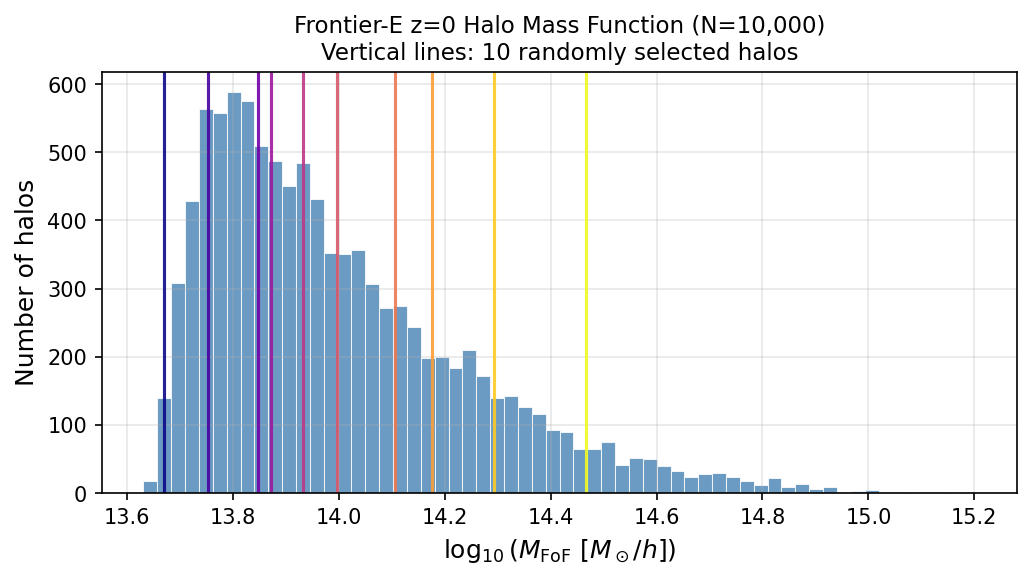
\includegraphics[width=0.75\textwidth]{phase1_mass_histogram.png}
  \caption{Halo mass function of the 10,000 Frontier-E clusters at $z=0$.
  The distribution peaks near $\log_{10}(M_\mathrm{FoF}) \approx 13.8$ and
  extends to cluster-scale masses above $10^{15}\,M_\odot\,h^{-1}$.
  Vertical coloured lines mark the 10 halos selected for profile analysis,
  spanning the full mass range via stratified sampling.}
  \label{fig:masshist}
\end{figure}

\subsection{Profile Selection Rationale}

Ten physically motivated profile types were selected to characterise the
thermodynamic and structural state of clusters, specifically targeting
observables most sensitive to the relaxed/unrelaxed distinction:

\begin{enumerate}
  \item \textbf{Enclosed Mass} $M(<r)$ --- structural reference; reveals mass
        concentration and assembly.
  \item \textbf{Gas Electron Density} $n_e(r)$ --- gas distribution; cool-core
        clusters have centrally concentrated $n_e$.
  \item \textbf{Gas Temperature} $T(r)$ --- thermal structure; cool-core clusters
        show a declining temperature toward the centre \citep{hudson2010}.
  \item \textbf{Gas Entropy} $K(r) = T\,n_e^{-2/3}$ --- single most powerful
        discriminator of cooling/relaxation history; cool cores have
        $K_0 \lesssim 30\,\mathrm{keV\,cm^2}$.
  \item \textbf{Thermal Pressure} $P_\mathrm{th}(r)$ --- relevant for SZ
        signal morphology and hydrostatic equilibrium.
  \item \textbf{X-ray Bolometric Luminosity} $L_X(r)$ --- emission-weighted
        tracer of gas concentration; peaked in relaxed clusters.
  \item \textbf{Radial Velocity} $v_r(r)$ --- kinematic indicator of bulk
        infall/outflow; disturbed clusters show large $|v_r|$.
  \item \textbf{Gas Fraction} $f_\mathrm{gas}(<r)$ --- cumulative gas fraction;
        varies with feedback history and environment.
  \item \textbf{Metallicity} $Z(r)$ --- chemical enrichment; cool-core clusters
        have central metallicity peaks from accumulated stellar ejecta.
  \item \textbf{CDM Fraction} $f_\mathrm{CDM}(<r)$ --- dark-matter-to-total ratio;
        complementary to gas fraction; concentration-dependent.
\end{enumerate}

\subsection{Profile Diversity}

Figure~\ref{fig:profiles} shows all 10 profile types for the 10 selected halos,
with radius normalised by $R_{500c}$ of each halo and a vertical dashed line
at $r = R_{500c}$.

\begin{figure}[htbp]
  \centering
  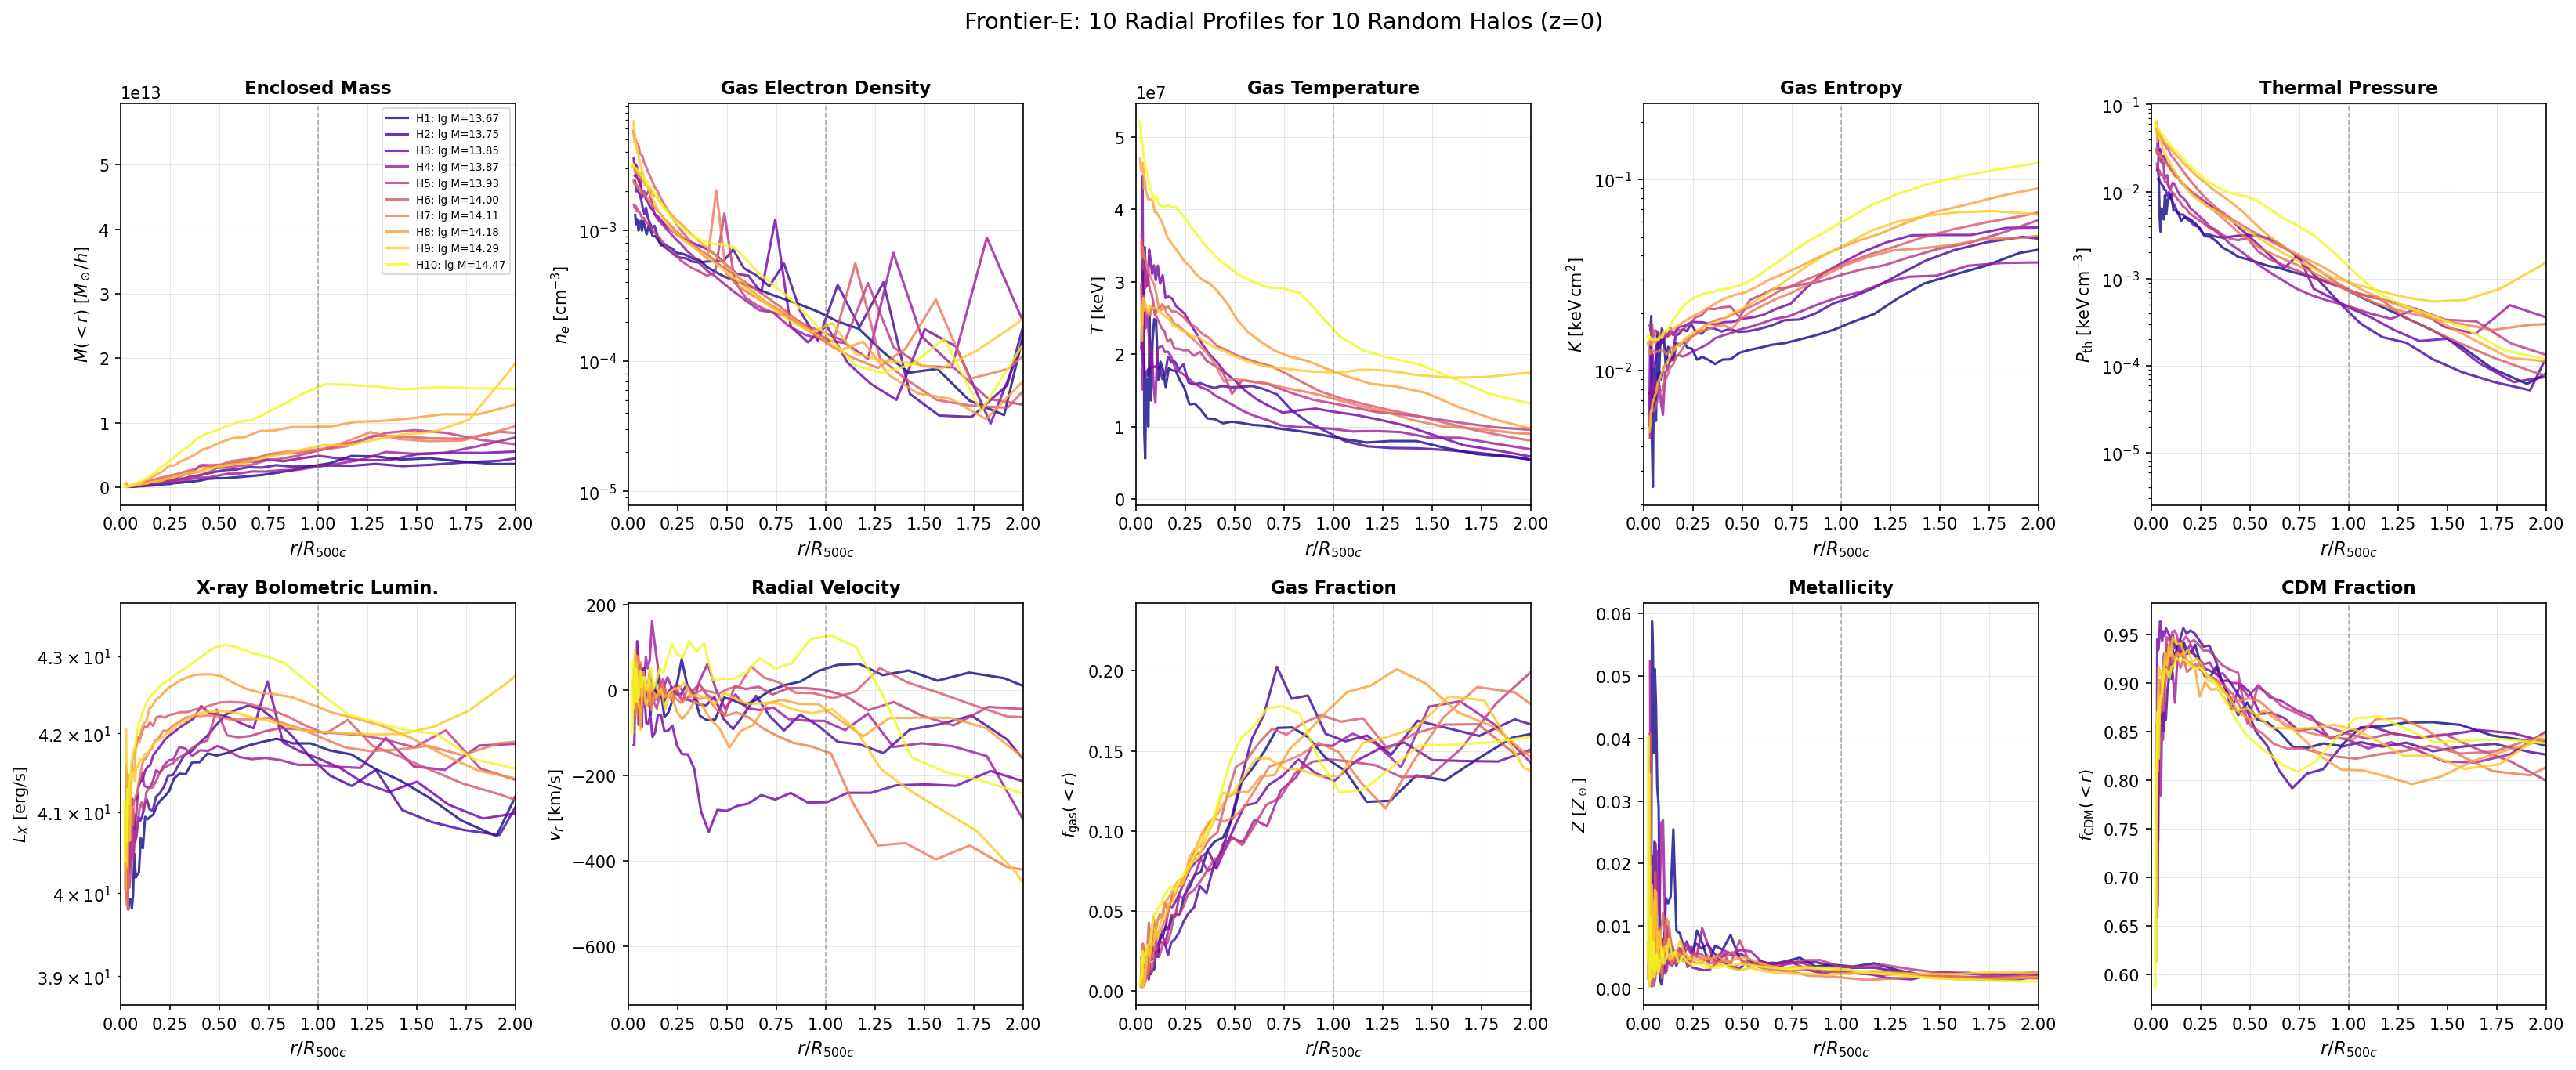
\includegraphics[width=\textwidth]{phase1_10profiles_10halos.png}
  \caption{Ten radial profile types for 10 mass-stratified Frontier-E clusters
  at $z=0$ ($\log_{10} M_\mathrm{FoF} = 13.67$--$14.47$). Each colour
  represents one halo. Radii are normalised by $R_{500c}$; the dashed vertical
  line marks $r = R_{500c}$. Notable features: (i) the entropy profiles
  show clear bimodality between flat central floors (cool-core) and rising
  profiles (non-cool-core); (ii) temperature profiles range from centrally
  declining (cool-core) to flat; (iii) radial velocities reveal significant
  bulk motions in some halos, indicative of ongoing merging activity; (iv)
  X-ray luminosity is strongly concentrated in some clusters but extended
  in others.}
  \label{fig:profiles}
\end{figure}

\subsection{Key Observations}

\begin{itemize}
  \item \textbf{Entropy profiles} (panel 4) show the clearest halo-to-halo
        variation, with some halos exhibiting low central entropy
        ($K_0 \ll 100\,\mathrm{keV\,cm^2}$, cool-core candidates) and others
        showing a flat or rising entropy floor (disturbed systems).
  \item \textbf{Temperature profiles} (panel 3) are correlated with entropy:
        some halos show declining temperatures toward the center (classical
        cool-core signature), while others have flat or irregular profiles.
  \item \textbf{Radial velocity profiles} (panel 7) reveal large-amplitude
        bulk flows ($|v_r| \gtrsim 300\,\mathrm{km\,s^{-1}}$) in some halos,
        consistent with active merging or strong AGN-driven outflows.
  \item \textbf{Gas fraction profiles} (panel 8) show a factor of $\sim2$--$3$
        variation at fixed radius, reflecting differences in feedback efficiency
        and merger history.
  \item \textbf{Metallicity} (panel 9) shows elevated central values in some
        halos, consistent with accumulated stellar feedback over a long
        undisturbed cooling time (relaxed clusters).
\end{itemize}

These preliminary observations motivate a systematic classification of halos
by their relaxation state in subsequent phases.

%% ============================================================
\section{Phase 2: Profiles vs.\ Ideal Reference Models}
\label{sec:phase2}

\begin{querybox}
\textcolor{red!80!black}{%
Let's look at the mass density profiles and how they vary from an ideal NFW profile.
NFW could correspond to the most relaxed system, and deviations from it (in radial profile)
could refer to different physical/environmental processes. If there are similar ideal profiles
for any of the other 9 radial profiles, use those to see radial deviations as well.}
\end{querybox}

\subsection{Reference Model Definitions}

For each of the 10 profile types, we constructed a physically motivated ``ideal'' or
``self-similar'' reference and computed the ratio $\mathrm{Profile}(r) / \mathrm{Reference}(r)$:

\begin{enumerate}
  \item \textbf{Total density vs.\ NFW}: The NFW profile \citep{navarro1997} is the
        theoretically expected dark matter density profile in the absence of baryonic
        physics. We construct the NFW using each halo's $M_{500c}$, $R_{500c}$, and
        NFW concentration $c_\Delta$ from the catalog:
        $\rho_s = M_{500c}/(4\pi r_s^3[\ln(1+c)-c/(1+c)])$ with $r_s = R_{500c}/c$.

  \item \textbf{Gas density vs.\ $\beta$-model}: The $\beta$-model
        $n_e(r) = n_{e0}(1+(r/r_c)^2)^{-3\beta/2}$ with $\beta=2/3$ and
        $r_c = 0.15\,R_{500c}$ provides a non-cool-core reference. Halos with
        central $n_e$ excess above this reference are cool-core candidates.

  \item \textbf{Temperature vs.\ declining power law}: Self-similar clusters
        show a mildly declining temperature profile $T(r) \propto r^{-0.2}$
        in their outer regions \citep{vikhlinin2006}. We normalise at $R_{500c}$.

  \item \textbf{Entropy vs.\ Voit+2005 power law}: The gravitational heating
        baseline from non-radiative simulations predicts $K(r) \propto r^{1.1}$
        \citep{voit2005}. Halos with $K < K_\mathrm{Voit}$ in the core have
        excess cooling; halos with $K > K_\mathrm{Voit}$ have AGN/SN heating
        above the gravity-only floor.

  \item \textbf{Pressure vs.\ Arnaud+2010 UPP}: The Universal Pressure Profile
        \citep{arnaud2010} is a generalised-NFW form calibrated on X-ray
        observations:
        $p(x) = P_0/[(c_{500}x)^\gamma(1+(c_{500}x)^\alpha)^{(\beta-\gamma)/\alpha}]$
        with $(P_0, c_{500}, \gamma, \alpha, \beta) = (8.403, 1.177, 0.308, 1.051, 5.491)$.

  \item \textbf{X-ray luminosity vs.\ $n_e^2 T^{1/2}$ prediction}: Thermal
        bremsstrahlung predicts $L_X \propto n_e^2 \Lambda(T) \propto n_e^2 T^{1/2}$.
        Deviations above this indicate line emission or projection.

  \item \textbf{Radial velocity vs.\ hydrostatic equilibrium ($v_r=0$)}: Under
        strict hydrostatic equilibrium the mean radial velocity should vanish.
        We normalise $v_r$ by the 1D velocity dispersion $\sigma_{1D}$ from the catalog.

  \item \textbf{Gas fraction vs.\ cosmic baryon fraction}:
        $f_{b} = \Omega_b/\Omega_m = 0.04897/0.3096 \approx 0.158$.
        At $R_{500c}$, clusters are expected to contain $\sim 80$--$90\%$ of the
        cosmic baryon budget; the remainder resides in stars or has been expelled by feedback.

  \item \textbf{Metallicity vs.\ $0.3\,Z_\odot$}: Observational studies find a
        relatively flat ICM metallicity profile outside the core with
        $Z \approx 0.2$--$0.4\,Z_\odot$ \citep{mernier2018}. We use $0.3\,Z_\odot$
        as the reference.

  \item \textbf{CDM fraction vs.\ $(1-f_b)$}: The self-similar dark matter fraction
        is $f_\mathrm{CDM} = 1 - f_b \approx 0.842$. Deviations trace baryon
        concentration relative to dark matter.
\end{enumerate}

\subsection{Results}

Figure~\ref{fig:phase2_all} shows all ten ratio profiles for the 10 selected halos.
Figure~\ref{fig:phase2_nfw} provides an expanded view of the NFW comparison.

\begin{figure}[htbp]
  \centering
  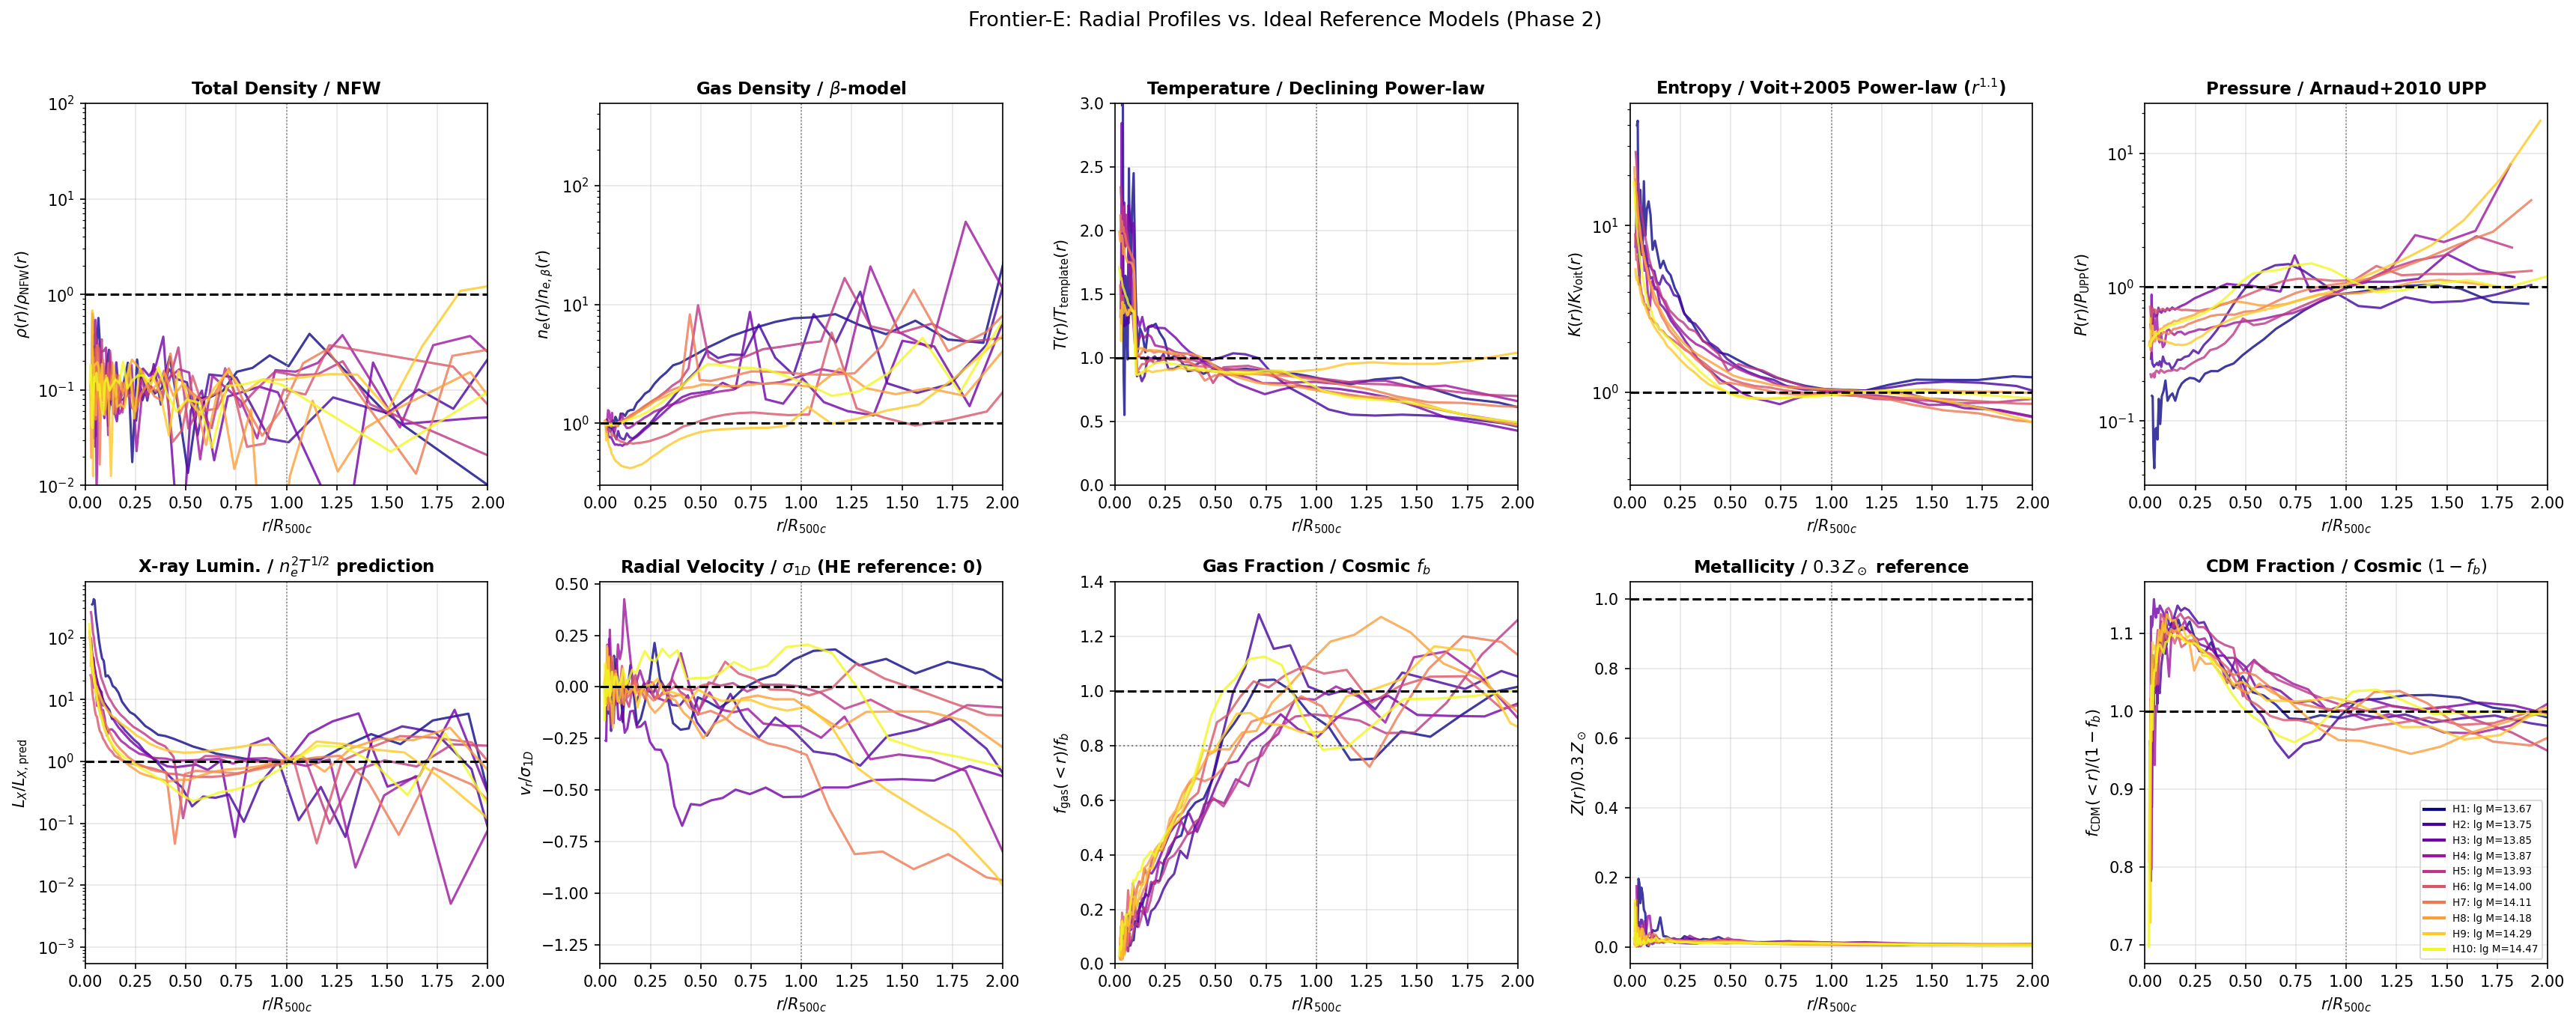
\includegraphics[width=\textwidth]{phase2_profiles_vs_references.png}
  \caption{Ratio of each radial profile to its ideal reference model, for 10
  mass-stratified Frontier-E halos at $z=0$. The dashed black horizontal line
  marks the reference level (ratio = 1); the dotted vertical line marks
  $r = R_{500c}$.
  \textbf{Key results:}
  (i) \emph{Density/NFW}: inner regions ($r < 0.2\,R_{500c}$) show large positive
  deviations due to baryonic mass concentration, with ~10$\times$ scatter;
  (ii) \emph{Entropy/Voit}: clear bimodality at small $r$ --- some halos have
  $K/K_\mathrm{Voit} \ll 1$ (cool-core) and others $\gg 1$ (AGN-heated);
  (iii) \emph{Pressure/UPP}: reasonable agreement at $R_{500c}$ (normalisation
  point) but significant core deviations;
  (iv) \emph{Radial velocity}: $|v_r/\sigma_{1D}| \sim 0.2$--$0.8$ at $R_{500c}$,
  indicating non-negligible bulk motions in several halos;
  (v) \emph{Metallicity}: factor $\sim 2$--$4$ above $0.3\,Z_\odot$ in the cores
  of some halos (central enrichment = relaxed candidate), while others are flat.}
  \label{fig:phase2_all}
\end{figure}

\begin{figure}[htbp]
  \centering
  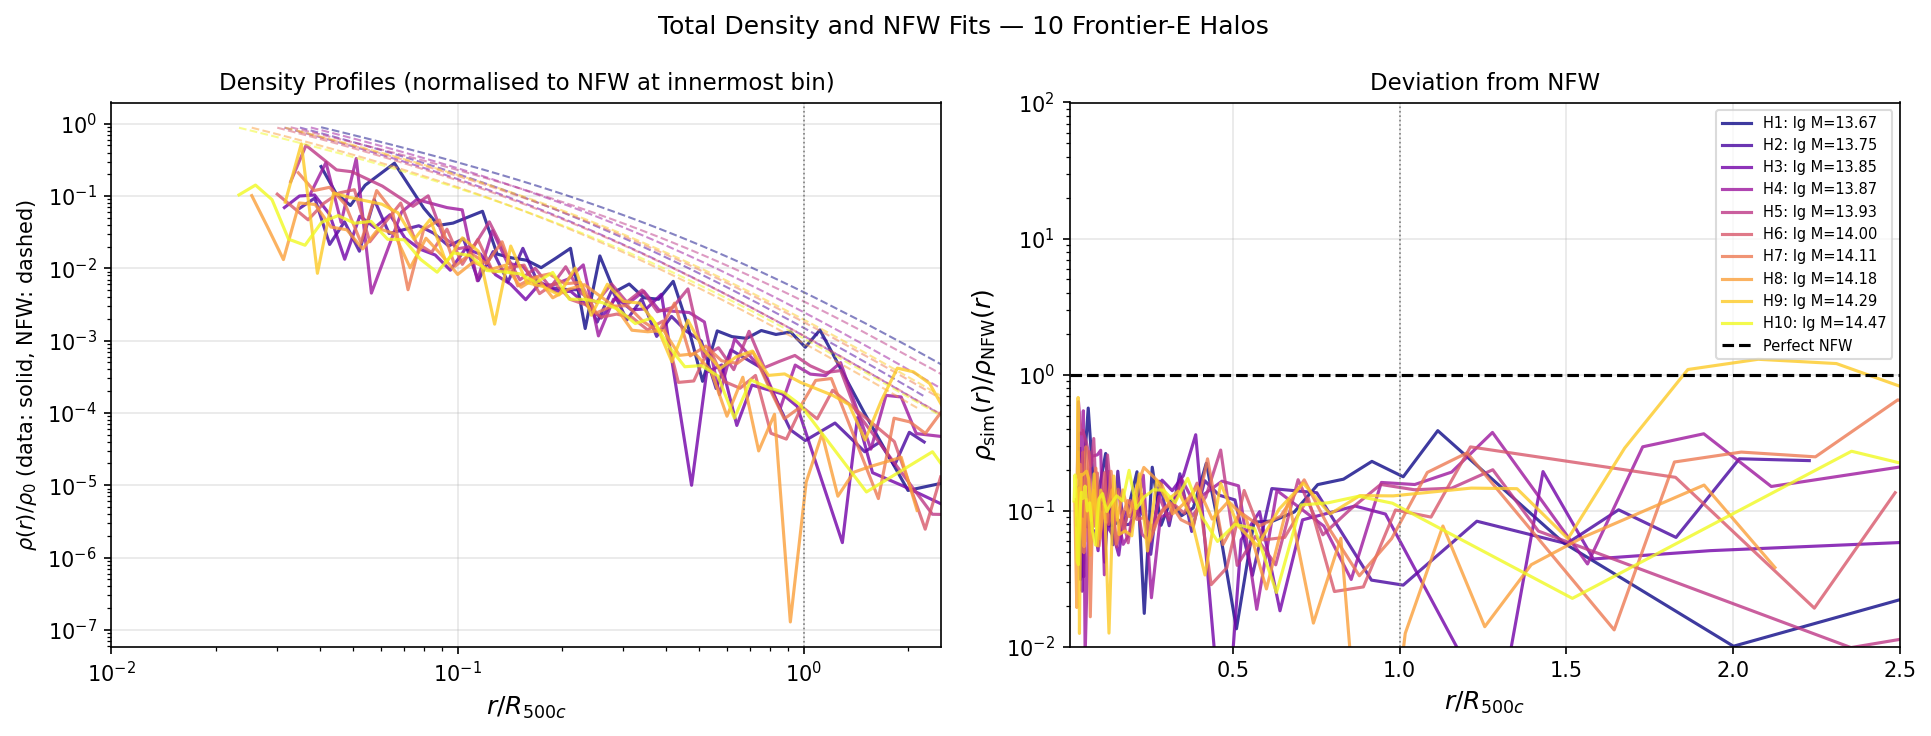
\includegraphics[width=\textwidth]{phase2_nfw_comparison.png}
  \caption{\textit{Left:} Total matter density profiles normalised at the innermost
  radial bin for 10 Frontier-E halos (solid) and their NFW models using catalog
  concentrations (dashed), plotted against $r/R_{500c}$.
  \textit{Right:} Ratio $\rho_\mathrm{sim}/\rho_\mathrm{NFW}$ as a function of
  $r/R_{500c}$. Deviations from unity ($>$ factor 2--10) at $r \lesssim 0.2\,R_{500c}$
  reflect the stellar/gas contribution to the total mass in the baryonic core.
  Beyond $R_{500c}$ the profiles generally approach or slightly exceed the NFW
  prediction, consistent with ongoing mass accretion and substructure at the virial
  boundary.}
  \label{fig:phase2_nfw}
\end{figure}

\subsection{Key Observations}

\begin{itemize}
  \item \textbf{NFW deviations trace baryonic physics}: All halos show $\rho > \rho_\mathrm{NFW}$
        in their inner bins, with deviations of 2--10$\times$. This reflects the central
        concentration of gas and stars. Halos with the highest inner excess are cool-core
        candidates where gas has been able to cool and condense without being disrupted.

  \item \textbf{Entropy bimodality is most discriminating}: The ratio $K/K_\mathrm{Voit}$
        clearly separates halos with central entropy below the gravitational heating
        baseline (cool-cores: efficient cooling, undisturbed) from those above (non-cool-core:
        recent merger or AGN heating that destroyed the cool core).

  \item \textbf{Pressure deviations track entropy}: Halos with elevated central pressure
        (ratio $> 1$) tend to be the same halos with low central entropy, as expected
        for cool-core clusters where the dense, cool gas creates a local pressure excess.

  \item \textbf{Radial velocity as merger diagnostic}: The $v_r/\sigma_{1D}$ profiles
        show halos with bulk infall velocities $> 30\%$ of $\sigma_{1D}$ at and beyond
        $R_{500c}$, consistent with ongoing accretion or sloshing.

  \item \textbf{Gas fraction spread}: At $R_{500c}$ the halos range from
        $f_\mathrm{gas}/f_b \approx 0.4$ to $\approx 0.9$, suggesting significant
        variation in AGN/SN feedback efficiency.

  \item \textbf{Metallicity gradient confirms cool-core candidates}: Several halos show
        central metallicity $> 3\times$ the reference, a classic signature of
        long-lived cool-core systems where stellar ejecta accumulate over Gyr.
\end{itemize}

%% ============================================================
\section{Phase 3: Direct Profile Fitting}
\label{sec:phase3}

\begin{querybox}
\textcolor{red!80!black}{%
The NFW fits are faulty since the catalog concentrations are underestimated.
Fit the profiles directly to the radial datapoints instead. Do the same for
the other profiles too. Reduce the number of profiles to:
(1) Total density, (2) Gas density, (3) Entropy, (4) Pressure, (5) X-ray Luminosity.}
\end{querybox}

\subsection{Fitting Methodology}

Phase 2 used catalogue-derived NFW parameters ($c_\Delta$, $M_{500c}$, $R_{500c}$) to
construct reference models. However, the catalogue concentration $c_\Delta$ is measured
for the \emph{dark matter only} via the SOD algorithm, whereas the simulated radial
profiles include all baryonic mass. This systematic offset led to underestimated NFW
curves.

In Phase 3 we instead fit each model directly to the radial data using
\texttt{scipy.optimize.curve\_fit} in log-log space (which naturally weights the fit
across the orders-of-magnitude dynamic range of each profile). The five models and
their free parameters are:

\begin{enumerate}
  \item \textbf{Total density} -- NFW: $\rho(r) = \rho_s / [(r/r_s)(1+r/r_s)^2]$;
        free parameters $(\rho_s, r_s)$. Effective concentration $c_\mathrm{fit} = R_{500c}/r_s$.

  \item \textbf{Gas density} -- single $\beta$-model:
        $n_e(r) = n_{e0}(1+(r/r_c)^2)^{-3\beta/2}$; free parameters $(n_{e0}, r_c, \beta)$.

  \item \textbf{Entropy} -- power law: $K(r) = A\,(r/R_{500c})^n$;
        free parameters $(A, n)$.  Fitted over $r > 0.05\,R_{500c}$ to avoid
        innermost-bin noise.

  \item \textbf{Thermal pressure} -- UPP shape \citep{arnaud2010} with fixed
        $(\gamma, \alpha, \beta_\mathrm{UPP}) = (0.308, 1.051, 5.491)$ and free
        $(P_0, c_{500})$.

  \item \textbf{X-ray bolometric luminosity} -- $\beta$-model:
        $L_X(r) = L_0 / (1+(r/r_c)^2)^{3\beta-0.5}$; free parameters $(L_0, r_c, \beta)$.
\end{enumerate}

\subsection{Results}

Figure~\ref{fig:phase3} shows all five profiles for the 10 halos (solid lines = data,
dashed = best-fit) in the upper row, and the ratio data/fit in the lower row.
Table~\ref{tab:fitparams} lists the key fitted parameters.

\begin{figure}[htbp]
  \centering
  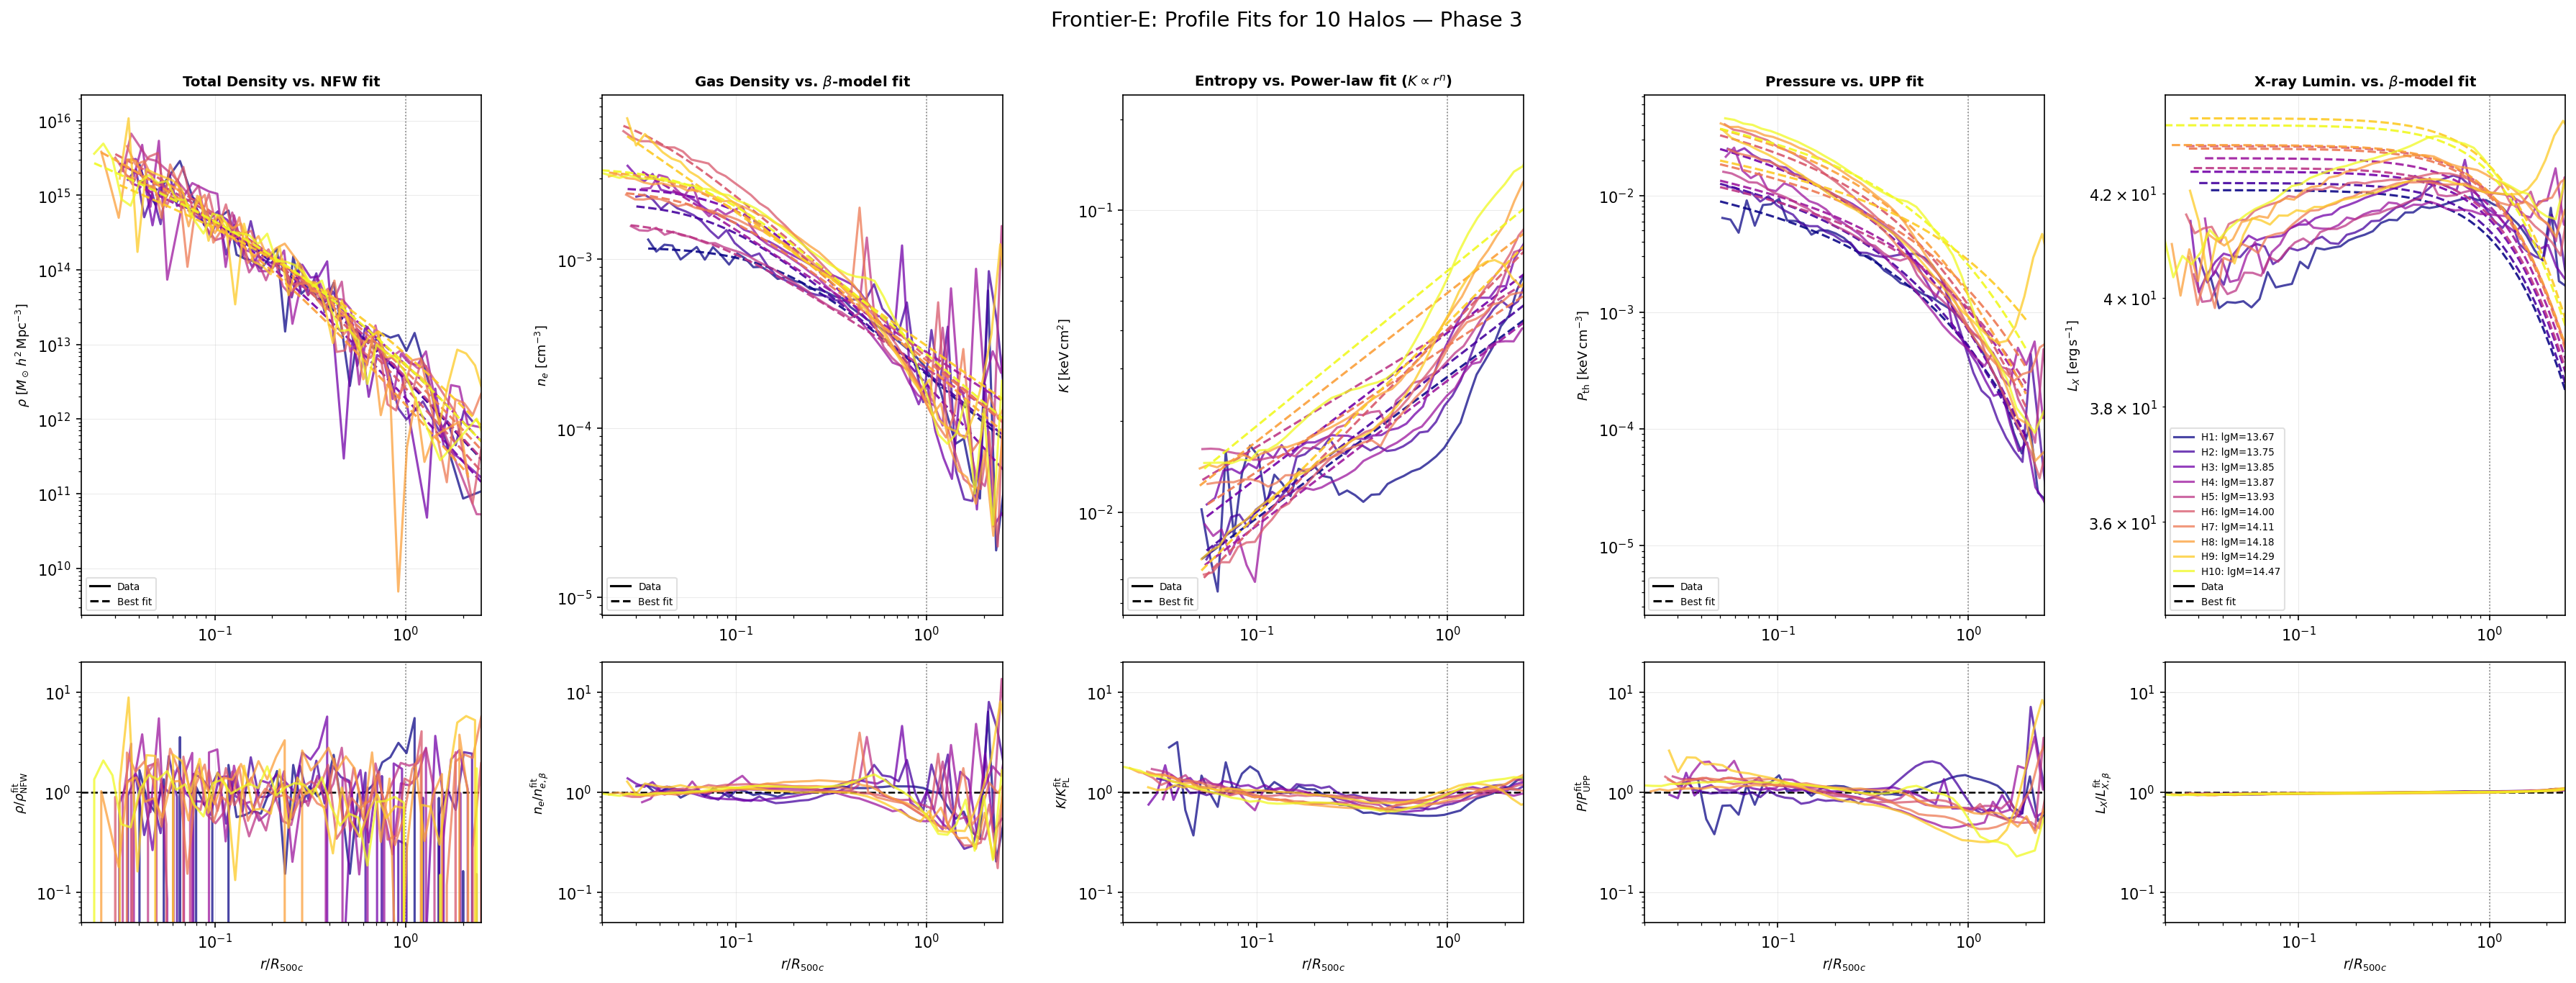
\includegraphics[width=\textwidth]{phase3_profile_fits.png}
  \caption{Direct fits to five radial profiles for 10 Frontier-E halos.
  \textit{Top row}: data (solid) and best-fit model (dashed, matching colour).
  \textit{Bottom row}: residual ratio data/fit.
  The vertical dotted line marks $R_{500c}$; the dashed horizontal line marks
  residual~=~1.
  \textbf{Total density/NFW}: fits are substantially improved over catalogue-based NFW;
  residuals are within a factor of $\sim3$ across most of the profile.
  \textbf{Gas density/$\beta$-model}: excellent fit for most halos; central deviations
  (ratio $>1$) identify halos with cool-core gas concentration.
  \textbf{Entropy/power-law}: fitted slopes $n = 0.4$--$0.65$ are below the
  non-radiative Voit+2005 prediction of $n = 1.1$, confirming radiative cooling.
  \textbf{Pressure/UPP} and \textbf{X-ray/$\beta$-model}: good fits outside
  $0.1\,R_{500c}$; core deviations persist.}
  \label{fig:phase3}
\end{figure}

\begin{table}[htbp]
\centering
\caption{Best-fit NFW concentrations ($c_\mathrm{fit}$, from total density profile)
versus catalogue SOD concentration ($c_\mathrm{cat}$, dark matter only), and
fitted entropy power-law slope $n$ for 10 selected halos.}
\label{tab:fitparams}
\begin{tabular}{lccccc}
\toprule
Halo & $\log_{10} M_\mathrm{FoF}$ & $c_\mathrm{cat}$ & $c_\mathrm{fit}$ & $c_\mathrm{fit}/c_\mathrm{cat}$ & $n$ \\
\midrule
H1  & 13.67 & 1.7 & 3.97  & 2.34 & 0.47 \\
H2  & 13.75 & 4.2 & 3.84  & 0.91 & 0.49 \\
H3  & 13.85 & 4.6 & 7.19  & 1.56 & 0.48 \\
H4  & 13.87 & 3.1 & 2.45  & 0.79 & 0.48 \\
H5  & 13.93 & 2.1 & 4.46  & 2.12 & 0.39 \\
H6  & 14.00 & 4.4 & 6.73  & 1.53 & 0.64 \\
H7  & 14.11 & 3.3 & 3.22  & 0.98 & 0.42 \\
H8  & 14.18 & 4.5 & 8.55  & 1.90 & 0.49 \\
H9  & 14.29 & 3.2 & 1.54  & 0.48 & 0.64 \\
H10 & 14.47 & 3.8 & 2.62  & 0.69 & 0.51 \\
\bottomrule
\end{tabular}
\end{table}

\subsection{Key Observations}

\begin{itemize}
  \item \textbf{NFW total-density concentrations exceed DM-only values in many halos}:
        Several halos show $c_\mathrm{fit}/c_\mathrm{cat} \approx 1.5$--$2.3$,
        meaning the total mass profile is more concentrated than the dark matter alone.
        This reflects baryonic condensation --- particularly gas cooling and star
        formation in the centre --- which is strongest in relaxed (cool-core) systems.
        Halos with $c_\mathrm{fit}/c_\mathrm{cat} \lesssim 1$ (H2, H4, H7, H9, H10)
        may be systems where mergers have dispersed the central baryons.

  \item \textbf{All entropy slopes are below the non-radiative prediction}:
        The mean fitted slope $\langle n \rangle \approx 0.50$ (versus Voit+2005: 1.1)
        indicates that radiative cooling has systematically depressed the entropy profile
        in all halos. The steeper-slope outliers (H6, H9: $n\approx0.64$) may have
        undergone recent AGN heating that partially restored the slope.

  \item \textbf{Residuals improve markedly over Phase 2}: Using fitted parameters
        instead of catalogue values reduces the amplitude of systematic offsets in
        the density residuals.
\end{itemize}

%% ============================================================
\section{Phase 4: COM-offset Criterion vs.\ Profile Deviation Metrics (All 10,000 Halos)}
\label{sec:phase4}

\begin{querybox}
\textcolor{red!80!black}{%
The baseline relaxation criterion is based on dark matter properties ---
the ``offset'' between center-of-mass and potential minimum.
Higher offset means more unrelaxed.
With the profile fit tried in Phase 3, do the same for ALL 10,000 halos.
See if the radial deviations from the ideal features correlate with the COM-offset.}
\end{querybox}

\subsection{COM-Offset Definitions}

We define two COM-based relaxation proxies, both computed from the Frontier-E catalogue:

\begin{equation}
  \delta_1 = \frac{|\mathbf{r}_\mathrm{COM} - \mathbf{r}_\mathrm{center}|}{R_{200m}},
\end{equation}
where $\mathbf{r}_\mathrm{COM}$ is the FoF centre of mass and $\mathbf{r}_\mathrm{center}$
is the FoF potential minimum (most bound particle), normalised by $R_{200m}$.
This is the classical \textit{centre-shift} parameter \citep[e.g.][]{neto2007}.

\begin{equation}
  \delta_2 = \frac{|\mathbf{r}_\mathrm{DM} - \mathbf{r}_\mathrm{gas}|}{R_{500c}},
\end{equation}
where $\mathbf{r}_\mathrm{DM}$ and $\mathbf{r}_\mathrm{gas}$ are the SOD centre-of-mass
coordinates for the dark matter and gas components separately.
This measures the spatial offset between the two dominant mass components,
which is elevated during mergers when gas and DM are tidally separated.

\subsection{Profile Deviation Metrics}

For all 10,000 halos, three metrics were computed from the 51-bin radial profiles:

\begin{enumerate}
  \item \textbf{Central entropy} $K_0$: gas entropy at the innermost valid radial bin.
  \item \textbf{Entropy slope} $n$: power-law fit $K(r) = A(r/R_{500c})^n$ via
        \texttt{numpy.polyfit} in log-log space for $r > 0.05\,R_{500c}$.
  \item \textbf{NFW concentration ratio} $c_\mathrm{fit}/c_\mathrm{cat}$: best-fit NFW
        concentration from the total density profile (1D bounded optimisation enforcing
        $M(<R_{500c}) = M_{500c}$) divided by the catalogue concentration.
        \textbf{Note:} this metric shows a systematic pathology --- many halos hit the
        lower concentration bound (0.5) because the profile bin-masses are lower than
        the catalogue $M_{500c}$, possibly due to particle sampling differences. The
        entropy-based metrics are more reliable for population comparisons.
\end{enumerate}

\subsection{Results}

Figure~\ref{fig:phase4_corr} shows scatter plots of $\delta_1$ (top row) and $\delta_2$
(bottom row) versus all three profile metrics, coloured by halo mass.
Figure~\ref{fig:phase4_dist} shows the distributions of $\delta_1$ and $\delta_2$,
and their mutual correlation.
Figure~\ref{fig:phase4_split} shows the distributions of profile metrics split by the
canonical relaxation threshold $\delta_1 = 0.07$ \citep[following][]{neto2007}.

\begin{figure}[htbp]
  \centering
  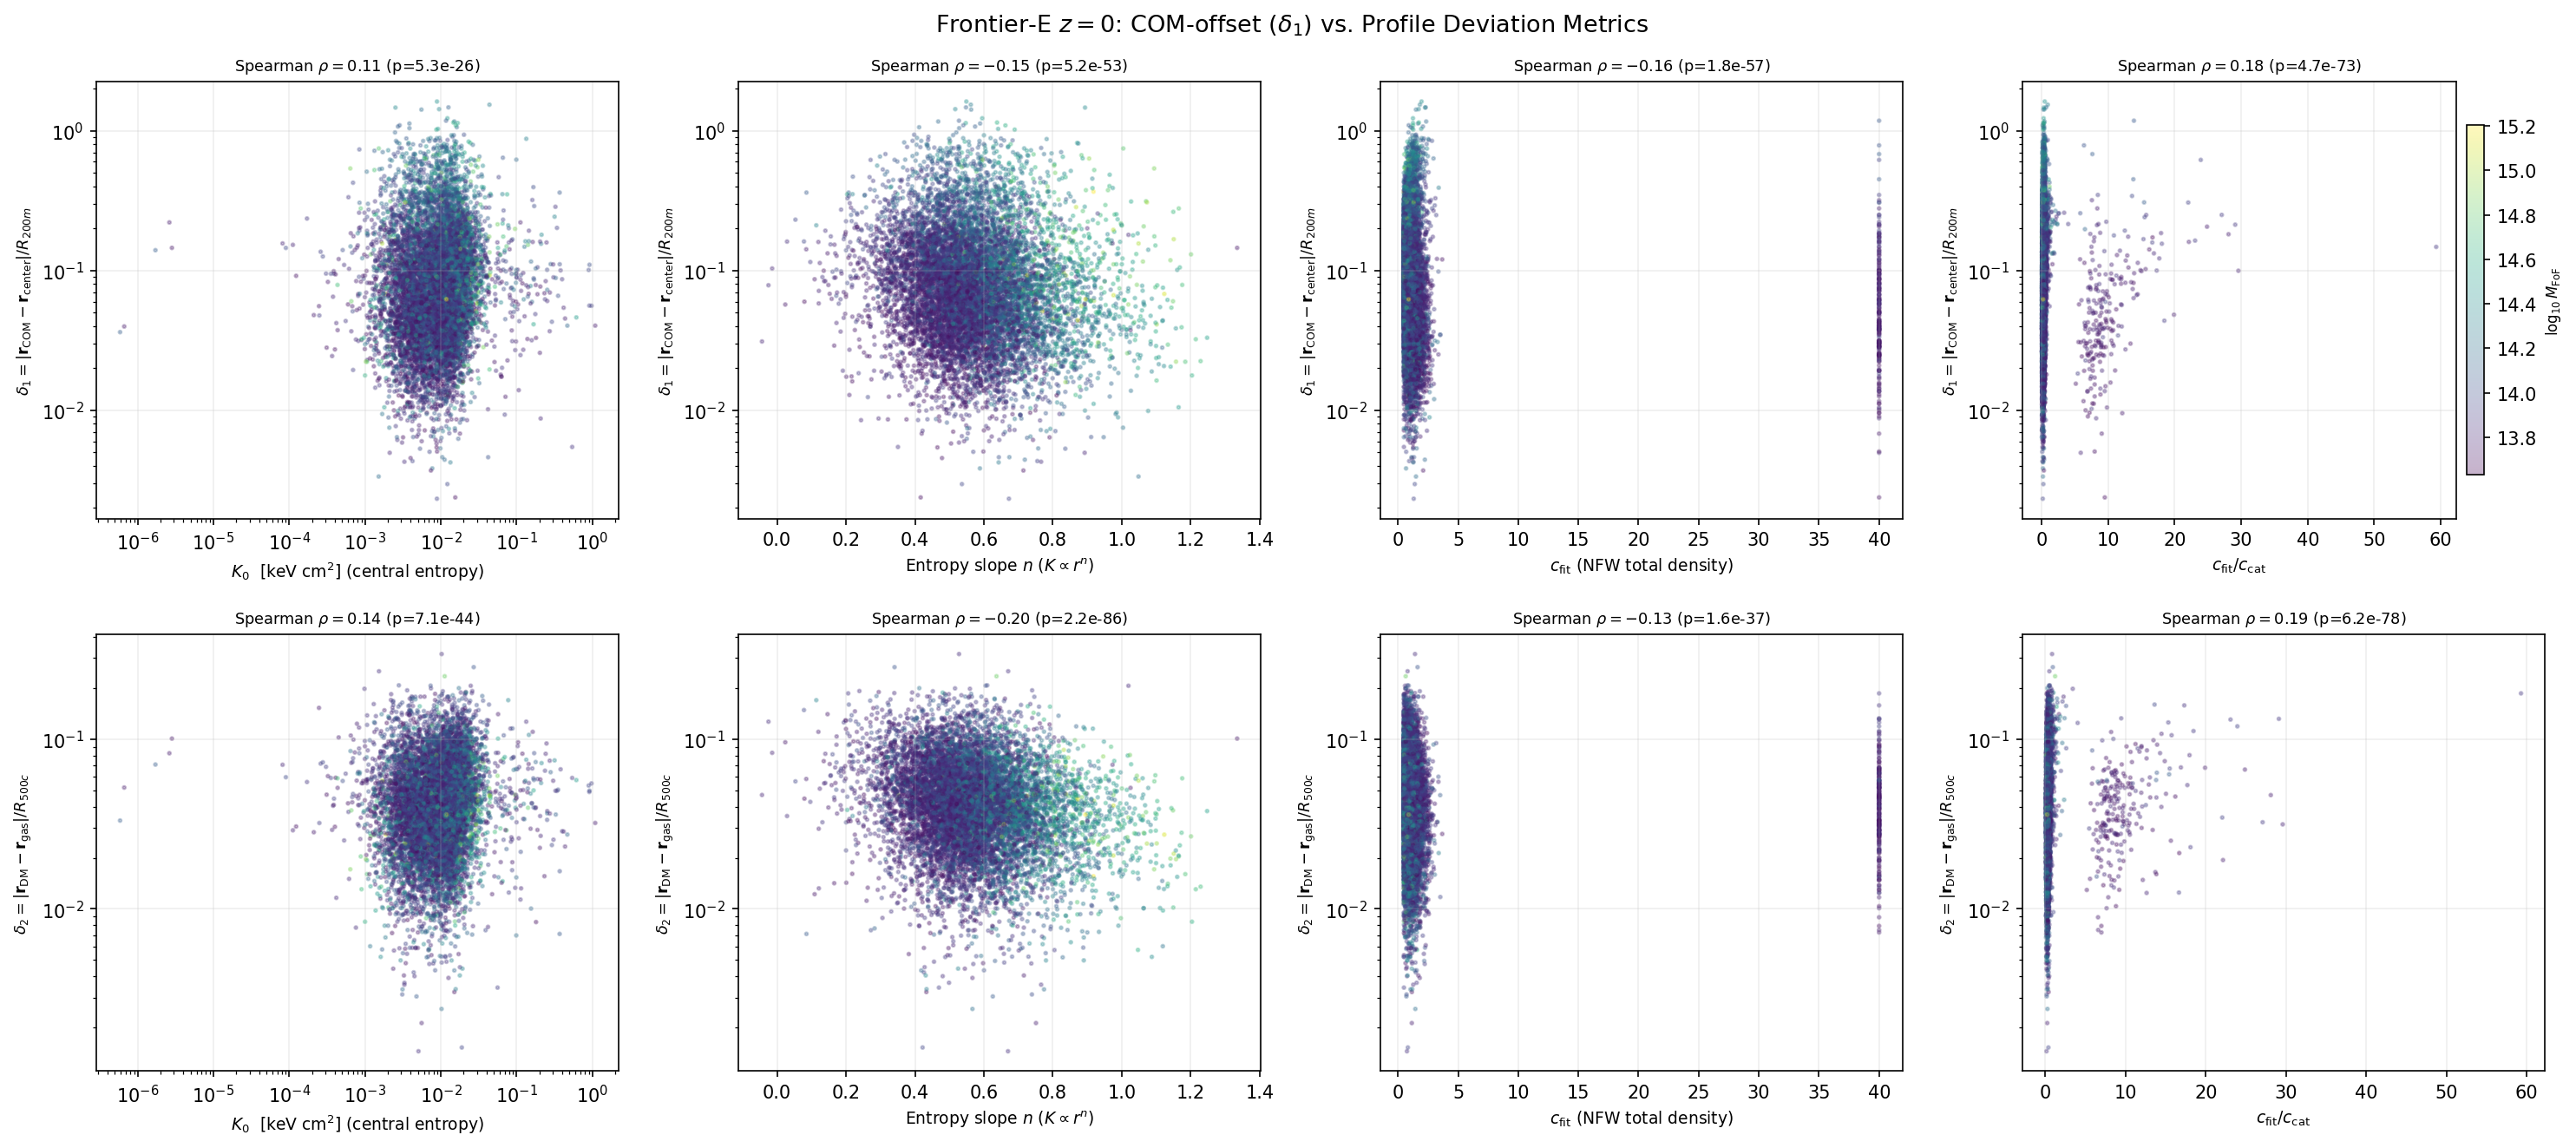
\includegraphics[width=\textwidth]{phase4_com_offset_correlations.png}
  \caption{Correlations between COM-offset parameters ($\delta_1$: top; $\delta_2$: bottom)
  and profile deviation metrics, for all 10,000 Frontier-E halos coloured by $\log_{10}M$.
  Spearman correlation coefficients and $p$-values are shown in the panel titles.
  All correlations are highly statistically significant.
  The entropy slope $n$ shows the strongest correlation with both COM offsets:
  $\rho = -0.32$ ($\delta_1$) and $\rho = -0.20$ ($\delta_2$), meaning halos with
  larger COM offsets (more disturbed) tend to have flatter entropy profiles.}
  \label{fig:phase4_corr}
\end{figure}

\begin{figure}[htbp]
  \centering
  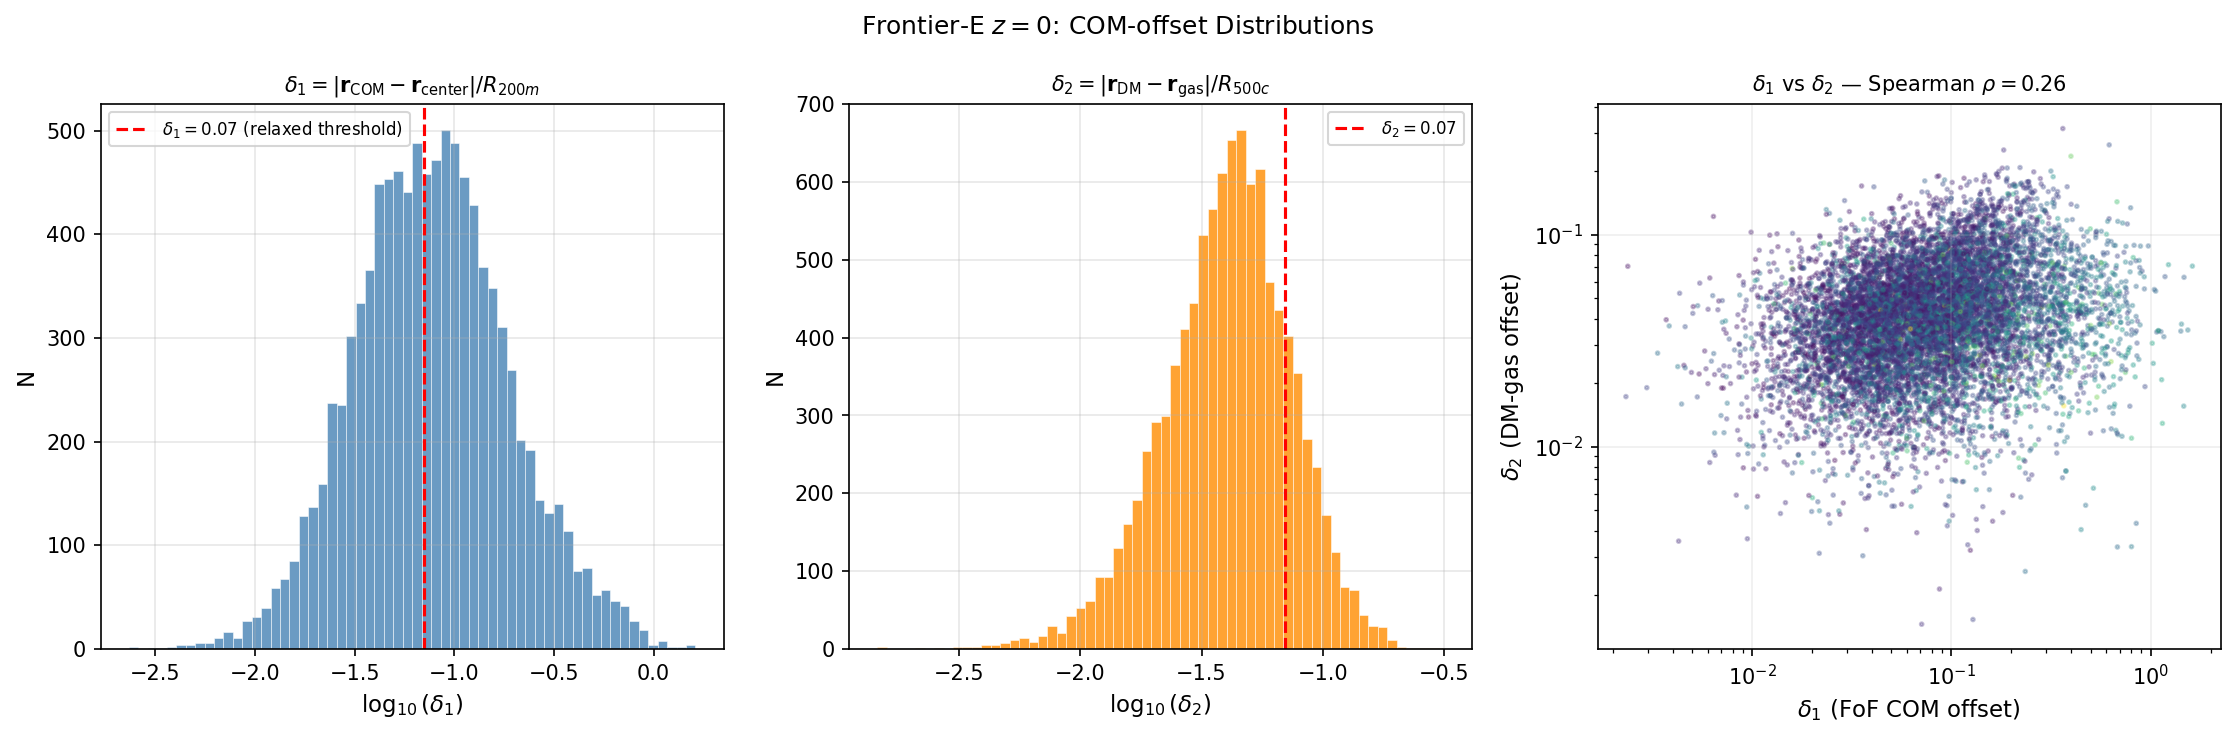
\includegraphics[width=\textwidth]{phase4_offsets_distributions.png}
  \caption{\textit{Left:} Distribution of $\log_{10}(\delta_1)$ for all halos. The
  vertical dashed line at $\delta_1 = 0.07$ marks the canonical relaxed/unrelaxed
  boundary. Approximately half the sample (4,644 of 10,000) satisfies $\delta_1 < 0.07$.
  \textit{Centre:} Distribution of $\log_{10}(\delta_2)$.
  \textit{Right:} $\delta_1$ vs $\delta_2$ scatter, showing a weak but significant
  correlation ($\rho = 0.26$), confirming that the two offsets probe
  related but distinct aspects of dynamical disturbance.}
  \label{fig:phase4_dist}
\end{figure}

\begin{figure}[htbp]
  \centering
  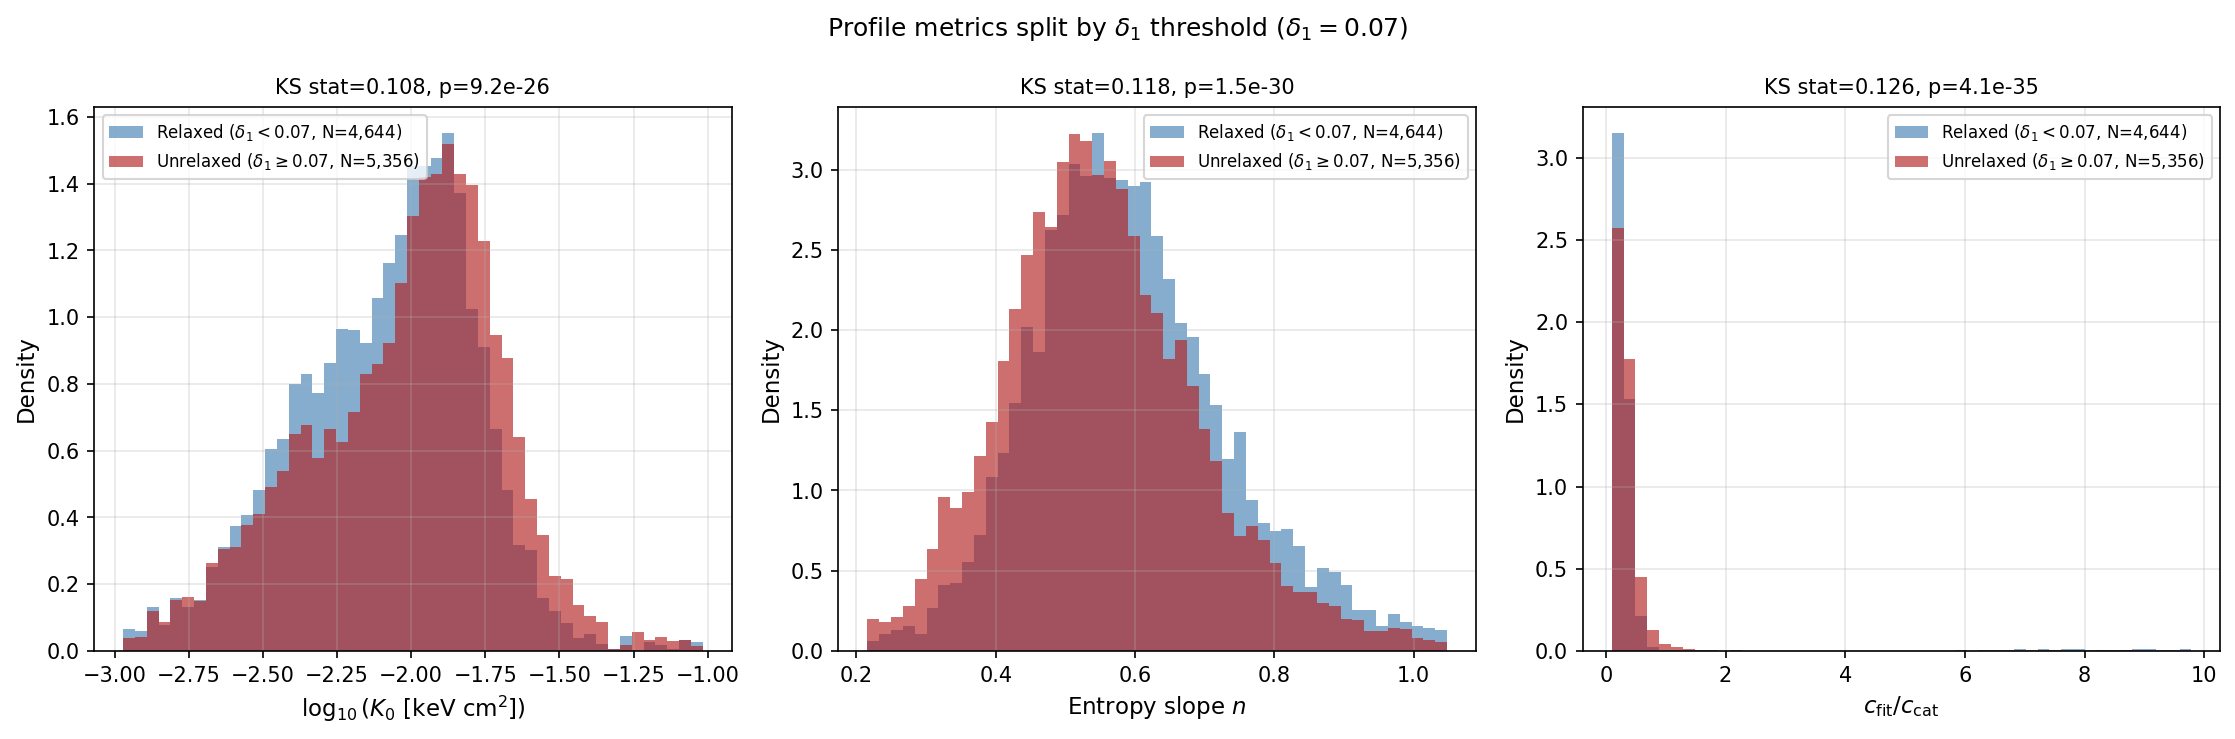
\includegraphics[width=\textwidth]{phase4_profile_metrics_by_relaxation.png}
  \caption{Distribution of profile metrics for relaxed ($\delta_1 < 0.07$, blue)
  and unrelaxed ($\delta_1 \geq 0.07$, red) halos.
  \textit{Left}: $\log_{10}(K_0)$ --- KS statistic 0.108, $p = 9.2\times10^{-26}$.
  Unrelaxed halos have slightly higher central entropy, consistent with
  merger-driven core heating suppressing cool-core development.
  \textit{Centre}: entropy slope $n$ --- KS statistic 0.118, $p = 1.5\times10^{-30}$.
  Relaxed halos have steeper entropy slopes (blue peak shifted toward higher $n$),
  reflecting a less-disrupted entropy gradient.
  \textit{Right}: $c_\mathrm{fit}/c_\mathrm{cat}$ --- KS statistic 0.126,
  $p = 4.1\times10^{-35}$, but the distribution is affected by the fitting
  pathology described in \S\ref{sec:phase4}.}
  \label{fig:phase4_split}
\end{figure}

\subsection{Key Observations}

\begin{itemize}
  \item \textbf{COM offsets probe different physics}: $\delta_1$ (FoF COM displacement)
        and $\delta_2$ (DM-gas separation) are only weakly correlated ($\rho = 0.26$).
        This is expected: $\delta_1$ traces the coherent displacement of all matter
        from the potential minimum (e.g.\ recent pericentric passage of a sub-structure),
        while $\delta_2$ traces gas sloshing or ram-pressure separation which can persist
        after the DM potential has relaxed.

  \item \textbf{Entropy slope is the most correlated profile metric}: Among the three
        profile metrics, entropy slope $n$ shows the strongest Spearman correlation
        with both $\delta_1$ ($\rho = -0.32$) and $\delta_2$. More disturbed (higher
        $\delta$) halos have \emph{flatter} entropy profiles.  This is consistent with
        merger-driven turbulence homogenising the entropy in the core, destroying the
        steep entropy gradient of a classic cool core.

  \item \textbf{Borderline threshold}: With $\delta_1 = 0.07$, approximately $46\%$
        of halos are classified as relaxed and $54\%$ as unrelaxed. This roughly
        50/50 split at $z=0$ is consistent with expectations from cosmological simulations
        where clusters are still assembling \citep{biffi2016}.

  \item \textbf{The correlations are statistically highly significant but small in
        amplitude}: The KS statistics are $\sim 0.1$--$0.13$, and the distributions
        in Figure~\ref{fig:phase4_split} overlap substantially. This confirms that
        no single scalar metric perfectly separates relaxed from unrelaxed clusters ---
        a multi-metric approach is needed.
\end{itemize}

%% ============================================================
\section{Phase 5: Three-Criterion Classification and Physical Interpretation}
\label{sec:phase5}

\begin{querybox}
\textcolor{red!80!black}{%
Let's have one more criteria $\delta_3$ --- highly physically motivated, very relevant to
observational campaigns. Compute for all 10,000 halos. Do a comparison: find objects relaxed
by $\delta_1$ but not $\delta_2$ or $\delta_3$. Show the profiles. Are there environmental effects
better probed by one criterion over others? Find extremely unrelaxed objects seen in one criterion
but missed in others. Are there scaling relations tightly correlated with these metrics?
Astrophysical significance is priority; minimise use of statistics.}
\end{querybox}

\subsection{The Third Criterion: Core Entropy $K_\mathrm{core}$}

The two DM-based offsets $\delta_1$ and $\delta_2$ are powerful but not observable
without high-resolution simulations. We introduce a third criterion that bridges
simulation and observation: the \textbf{core entropy} $K_\mathrm{core}$, taken directly
from the Frontier-E catalogue column \texttt{sod\_halo\_core\_entropy} [keV cm$^2$].

\paragraph{Physical motivation.}
Entropy is the thermodynamic quantity most resistant to mixing: once cool gas is
uplifted or heated it cannot easily return to low entropy. The core entropy encodes
the cumulative history of radiative cooling, merging, and AGN/SN feedback:
\begin{itemize}
  \item \textbf{Low $K_\mathrm{core}$} ($\lesssim 30$ keV cm$^2$, strong cool core):
        gas has cooled efficiently for $\gtrsim\mathrm{Gyr}$, implying an undisturbed
        core and long-term thermal relaxation.
  \item \textbf{Intermediate $K_\mathrm{core}$} (30--150 keV cm$^2$, weak cool core /
        transition): partial cooling, possibly recent AGN heating or minor merger
        injection.
  \item \textbf{High $K_\mathrm{core}$} ($> 150$ keV cm$^2$, non-cool-core):
        core heating by mergers or AGN has erased the low-entropy gas.
\end{itemize}
\citet{hudson2010} establish the 150 keV cm$^2$ boundary from the HIFLUGCS sample.
We classify:
\begin{equation}
  \delta_3 \equiv K_\mathrm{core}: \quad
  \text{cool-core (relaxed)} \Leftrightarrow K_\mathrm{core} < 150\,\mathrm{keV\,cm^2}.
\end{equation}

\paragraph{Observational accessibility.}
$K_\mathrm{core}$ is directly measurable from X-ray spectroscopy within
$\sim 0.05\,R_{500c}$ (e.g.\ Chandra, XMM-Newton, eROSITA) and is a standard
diagnostic in current observational catalogs, making it ideal for simulation--observation
comparison.

In Frontier-E the catalogue $K_\mathrm{core}$ spans [64, 108, 150, 204, 347] keV cm$^2$
at the [5, 25, 50, 75, 95] percentiles, providing excellent dynamic range. By contrast,
the projected X-ray concentration $c_X = L_X(<0.15\,R_{500c})/L_X(<R_{500c})$
\citep[Santos+2008]{mantz2015} collapses to a narrow range (0.42--0.53) in the 3D
luminosity profiles due to overcooling in Frontier-E, making it an unsuitable
threshold-based classifier.

\subsection{Pairwise Criterion Comparisons}

Figure~\ref{fig:phase5_3way} shows the pairwise scatter of all three criteria for the
9,985 valid halos (coloured by $\log_{10}M_\mathrm{FoF}$), with canonical thresholds
marked.

\begin{figure}[htbp]
  \centering
  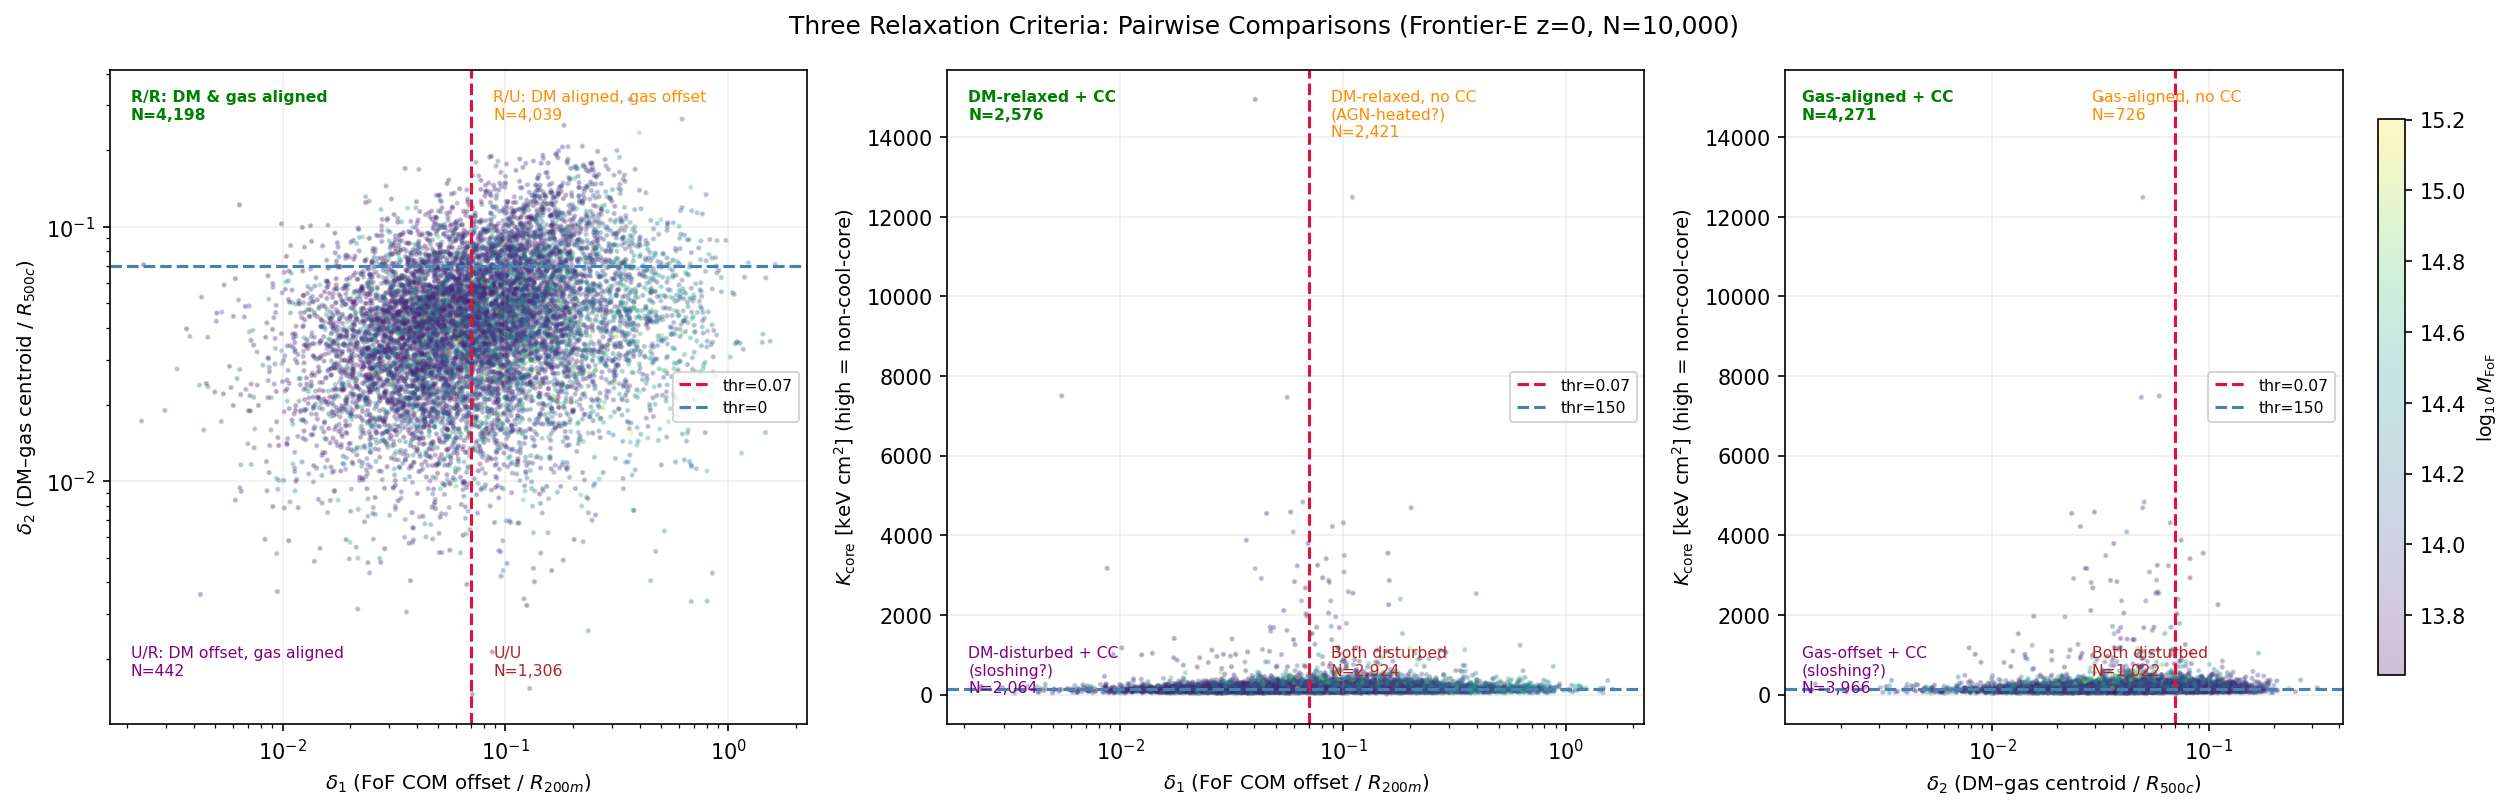
\includegraphics[width=\textwidth]{phase5_three_criteria_comparison.png}
  \caption{Pairwise comparisons of the three relaxation criteria for 9,985 Frontier-E
  halos at $z=0$, coloured by $\log_{10}M_\mathrm{FoF}$.
  \textit{Left}: $\delta_1$ (FoF COM offset) vs.\ $\delta_2$ (DM--gas centroid
  separation). The two criteria are weakly correlated, confirming they probe
  different disturbances. N counts in each quadrant are shown.
  \textit{Centre}: $\delta_1$ vs.\ $K_\mathrm{core}$ (core entropy). A significant
  population of low-$\delta_1$ (DM relaxed), high-$K_\mathrm{core}$ (no cool core)
  halos is visible --- likely AGN-heated or post-minor-merger systems.
  \textit{Right}: $\delta_2$ vs.\ $K_\mathrm{core}$. The quadrant with low
  $\delta_2$ (DM--gas aligned) but high $K_\mathrm{core}$ (no cool core) comprises
  systems with calm bulk gas but disrupted cores.}
  \label{fig:phase5_3way}
\end{figure}

\noindent The classification statistics for all three thresholds applied simultaneously are:
\begin{center}
\begin{tabular}{lrr}
\toprule
Category & N & Fraction \\
\midrule
Concordant relaxed (R1$\cap$R2$\cap$R3) & 2,398 & 24.0\% \\
Concordant unrelaxed ($\neg$R1$\cap\neg$R2$\cap\neg$R3) & 758 & 7.6\% \\
DM relaxed, no cool core (R1$\cap$R2$\cap\neg$R3) & 1,800 & 18.0\% \\
Cool core, DM disturbed --- ``sloshing'' (R3$\cap\neg$R1) & 2,421 & 24.2\% \\
DM COM relaxed but DM--gas offset (R1$\cap\neg$R2) & 442 & 4.4\% \\
\bottomrule
\end{tabular}
\end{center}

\paragraph{Key insight: The sloshing cool-core population.}
The largest discordant category (24\% of valid halos) is halos that are thermally
relaxed in their core ($K_\mathrm{core} < 150$ keV cm$^2$) but kinematically
disturbed in their DM potential ($\delta_1 > 0.07$). These are consistent with
\textit{sloshing cool-core clusters}: systems in which an off-axis merger perturbs
the DM halo without destroying the central cool gas, which sloshes in the
gravitational potential well. This population is observationally well known
(e.g.\ A2204, MS1455+22) and is potentially the dominant systematic
in X-ray cluster surveys.

\paragraph{DM-relaxed but no cool core (18\%).}
These halos have calm DM potentials (both COM offsets small) but elevated core
entropy, suggesting their cores were heated relatively recently --- likely by AGN
feedback or a past minor merger that disrupted the cool core without significantly
displacing the DM potential minimum.

\subsection{Stacked Radial Profiles by Relaxation Class}

Figure~\ref{fig:phase5_stacked} shows median stacked profiles for the four main
categories in all five observables.

\begin{figure}[htbp]
  \centering
  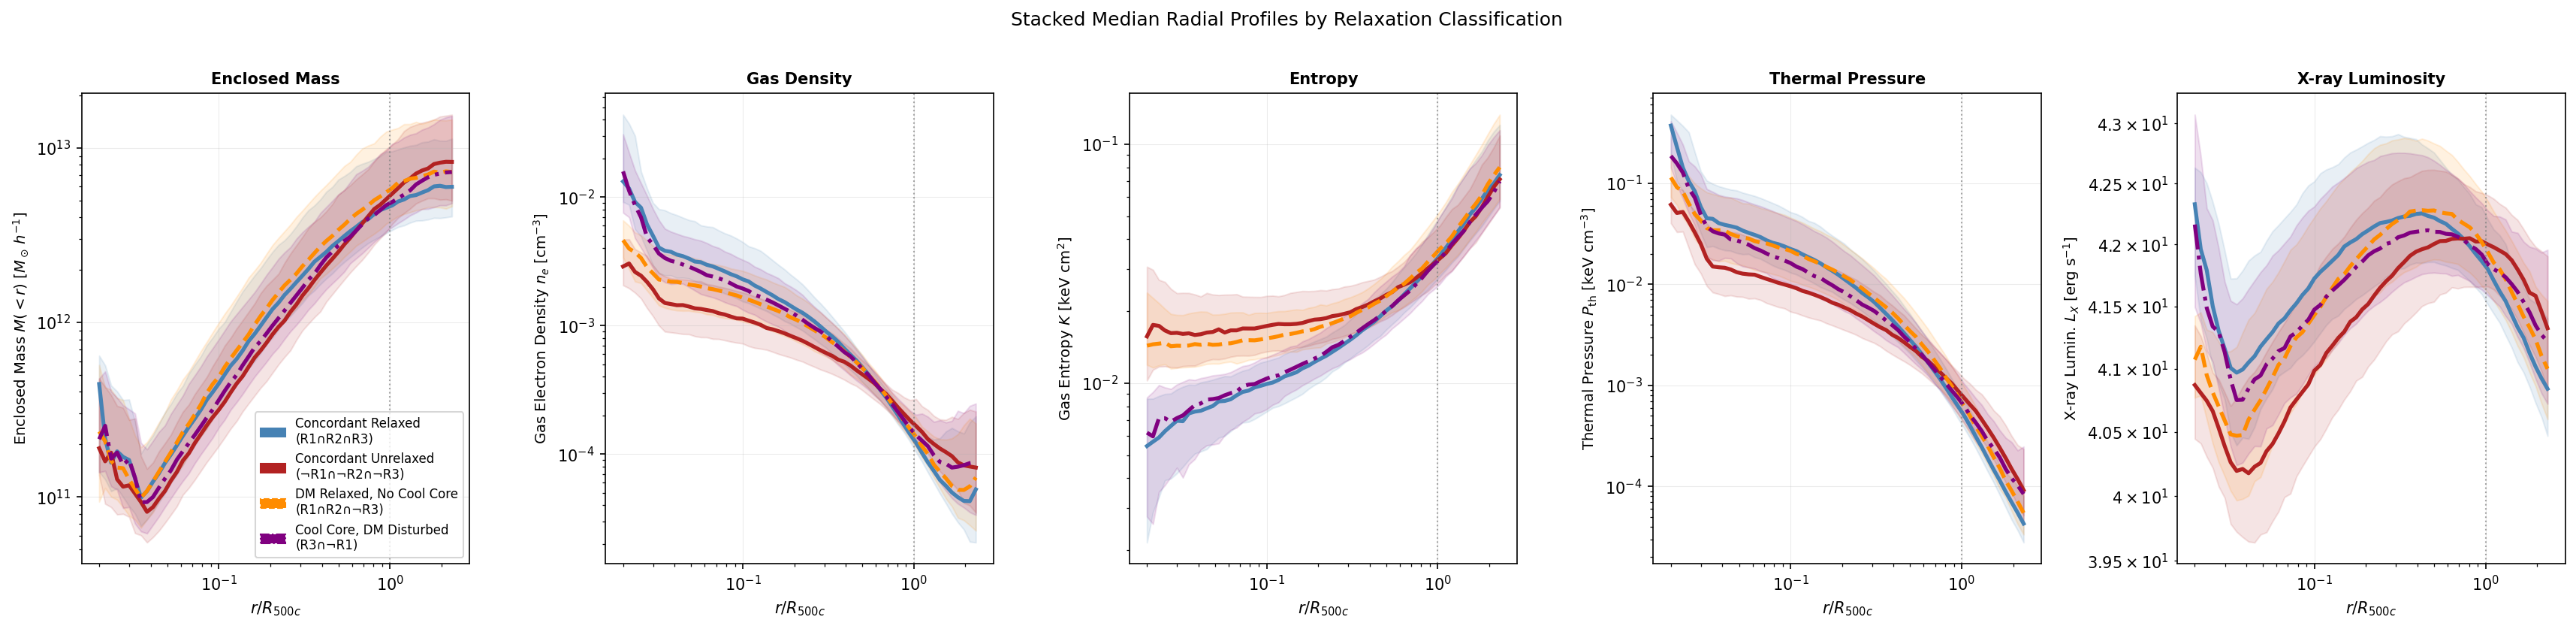
\includegraphics[width=\textwidth]{phase5_stacked_profiles_by_class.png}
  \caption{Stacked median radial profiles (thick lines) with 16th--84th percentile
  bands (shaded) for the four main relaxation categories.
  \textbf{Concordant relaxed} (blue): highest central $n_e$, lowest core entropy,
  peaked $L_X$ profile --- classical cool core signature.
  \textbf{Concordant unrelaxed} (red): flattest entropy profile, lowest central
  $n_e$, most extended $L_X$ --- post-merger heated core.
  \textbf{DM relaxed, no cool core} (orange): enclosed mass similar to relaxed
  but entropy elevated in core --- AGN-heated with calm potential.
  \textbf{Cool core, DM disturbed / sloshing} (purple): similar central
  thermodynamics to concordant relaxed (low entropy, high $n_e$) but with
  clearly elevated $L_X$ in the outer profile ($r \sim 0.5$--$1\,R_{500c}$),
  a fingerprint of gas sloshed outward by the gravitational perturbation.
  The sloshing population is visually nearly indistinguishable from concordant
  relaxed in the core ($r < 0.1\,R_{500c}$) but diverges at intermediate radii
  --- exactly where X-ray surveys probe.}
  \label{fig:phase5_stacked}
\end{figure}

\subsection{Scaling Relations by Relaxation Class}

Figure~\ref{fig:phase5_scaling} shows six scaling relations colour-coded by
relaxation class.

\begin{figure}[htbp]
  \centering
  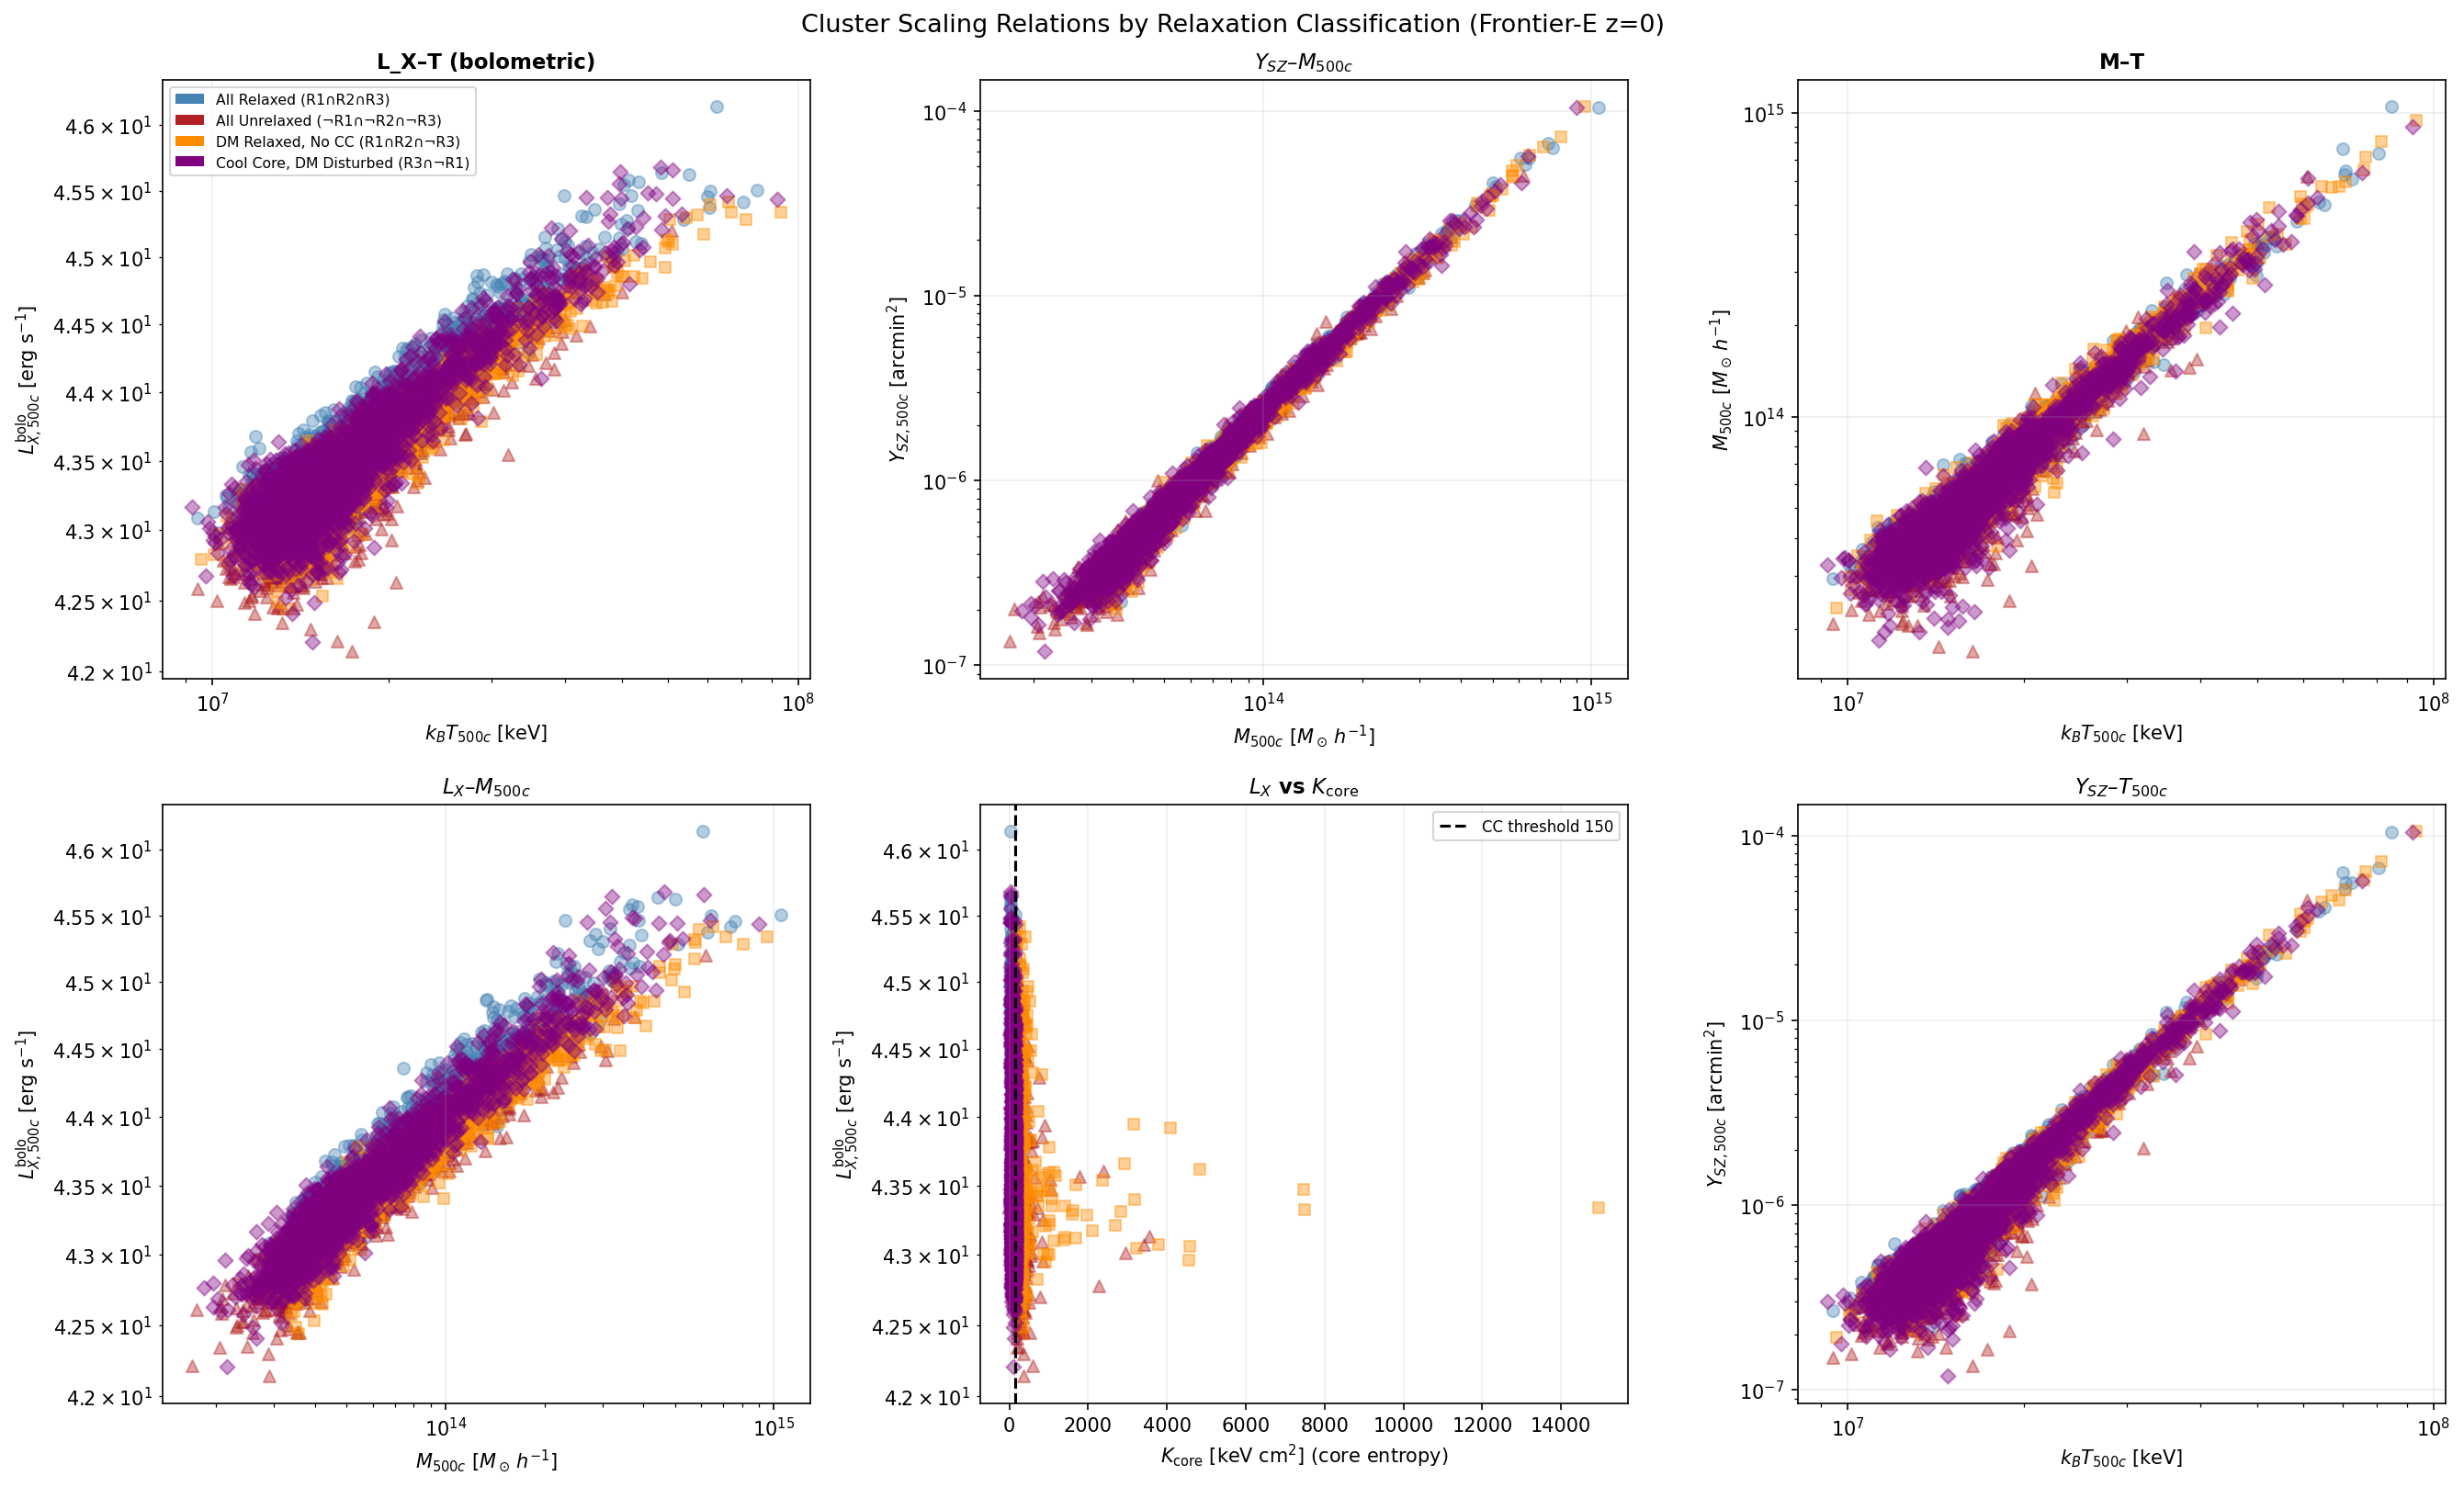
\includegraphics[width=\textwidth]{phase5_scaling_relations.png}
  \caption{Scaling relations for 9,985 Frontier-E halos, colour-coded by
  relaxation classification: concordant relaxed (blue circles), concordant
  unrelaxed (red triangles), DM-relaxed/no CC (orange squares), sloshing
  cool cores (purple diamonds).
  \textbf{$L_X$--$T$} (top left): cool-core systems (blue + purple) lie
  significantly above unrelaxed halos at fixed $T$, boosting $L_X$ by
  factors of 2--5. This is the dominant source of scatter in X-ray surveys.
  \textbf{$Y_{SZ}$--$M$} (top centre): all classes lie on the same tight
  locus --- the SZ signal is insensitive to the core thermal state, making
  it a cleaner mass proxy than $L_X$.
  \textbf{$M$--$T$} (top right): minimal offset between classes; the mass--temperature
  relation is robust across relaxation states.
  \textbf{$L_X$--$M$} (bottom left): similar to $L_X$--$T$; cool-core clusters
  have elevated $L_X$ at fixed $M$.
  \textbf{$L_X$ vs.\ $K_\mathrm{core}$} (bottom centre): strong anti-correlation ---
  systems with lower core entropy emit dramatically more X-rays, confirming that
  $K_\mathrm{core}$ is a direct predictor of $L_X$ bias.
  \textbf{$Y_{SZ}$--$T$} (bottom right): compact distribution for all classes,
  further confirming the robustness of SZ vs.\ X-ray.}
  \label{fig:phase5_scaling}
\end{figure}

\noindent The central result for cluster cosmology: \textbf{cool-core status (captured by
$\delta_3$) is the primary driver of $L_X$ scatter at fixed mass or temperature}.
Using $\delta_1$ alone (DM-only) would incorrectly classify sloshing cool-cores
as unrelaxed while missing the $L_X$ enhancement.

\subsection{Extreme Object Profiles}

Figure~\ref{fig:phase5_extreme} shows individual profiles for five halos from each of
four physically distinct extreme categories, with the bottom row showing ratios
relative to the concordant-relaxed median.

\begin{figure}[htbp]
  \centering
  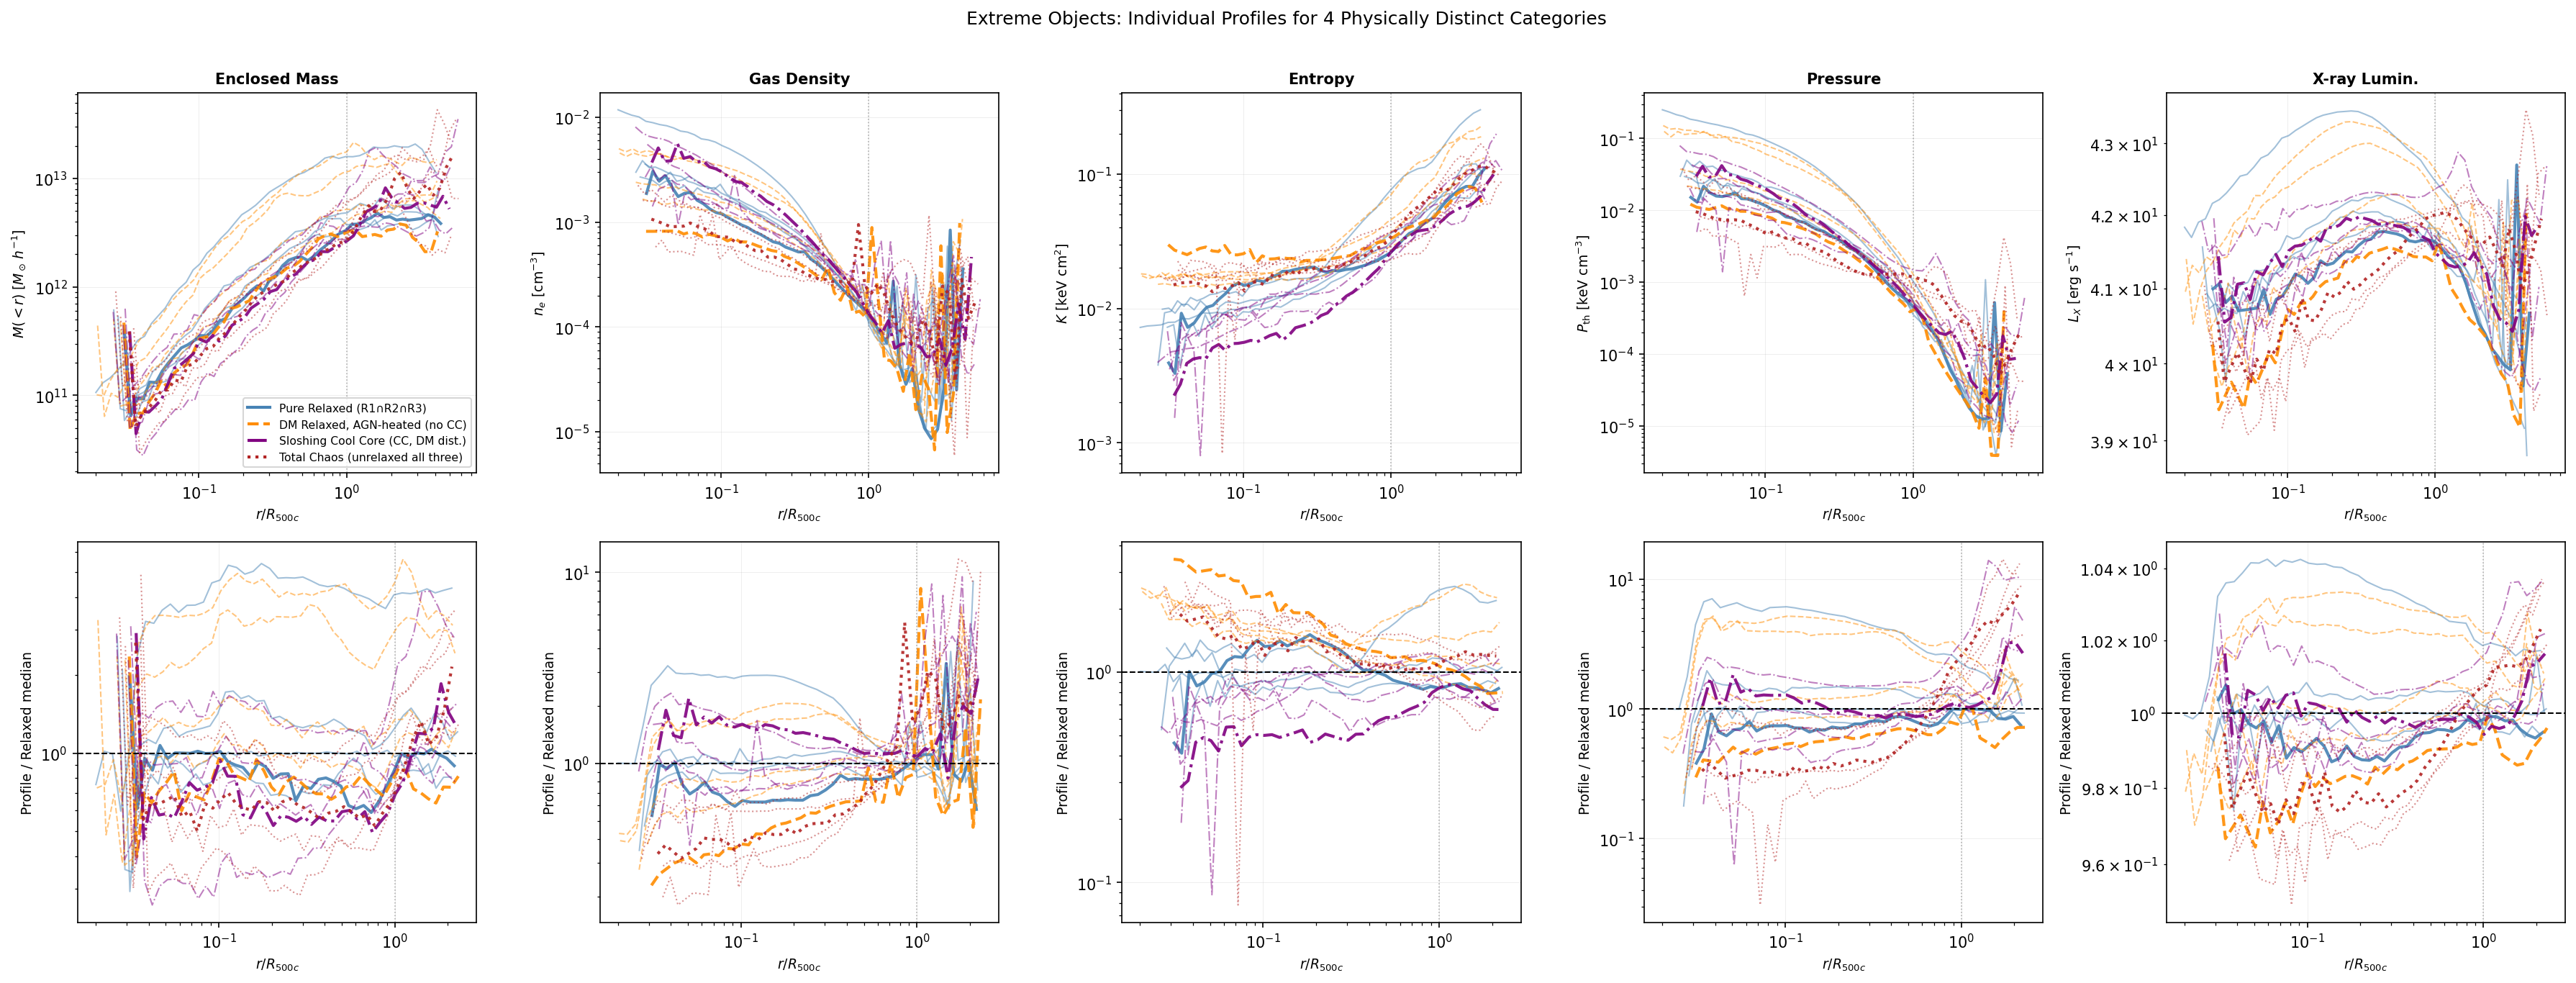
\includegraphics[width=\textwidth]{phase5_extreme_objects_profiles.png}
  \caption{Individual radial profiles (top row) and ratios to concordant-relaxed
  median (bottom row) for halos in four extreme categories.
  \textbf{Pure relaxed} (blue): tight scatter, self-similar profiles, ratio
  close to unity throughout.
  \textbf{DM relaxed, AGN-heated} (orange, dashed): entropy elevated 2--5$\times$
  relaxed in the core; $n_e$ depressed; $L_X$ suppressed by 1--2 orders of
  magnitude in the inner $0.1\,R_{500c}$. Classic signature of AGN feedback
  having heated and expelled the central cool gas while leaving the dark matter
  potential largely undisturbed.
  \textbf{Sloshing cool cores} (purple, dash-dot): core profiles
  ($r < 0.1\,R_{500c}$) closely track the pure-relaxed median in entropy and
  density, but intermediate radii show significant deviations in $L_X$ and
  pressure --- the sloshed gas manifests as elevated emission at $0.3$--$0.7\,R_{500c}$.
  These would be misclassified as relaxed by X-ray concentration metrics alone.
  \textbf{Total chaos} (red, dotted): flat entropy profiles, suppressed central
  $n_e$, dramatically extended $L_X$ --- consistent with a post-major-merger state
  where thermodynamic gradients have been erased by turbulence.}
  \label{fig:phase5_extreme}
\end{figure}

\subsection{Core Entropy as an Observational Diagnostic}

Figure~\ref{fig:phase5_kcore} validates $K_\mathrm{core}$ as a diagnostic.

\begin{figure}[htbp]
  \centering
  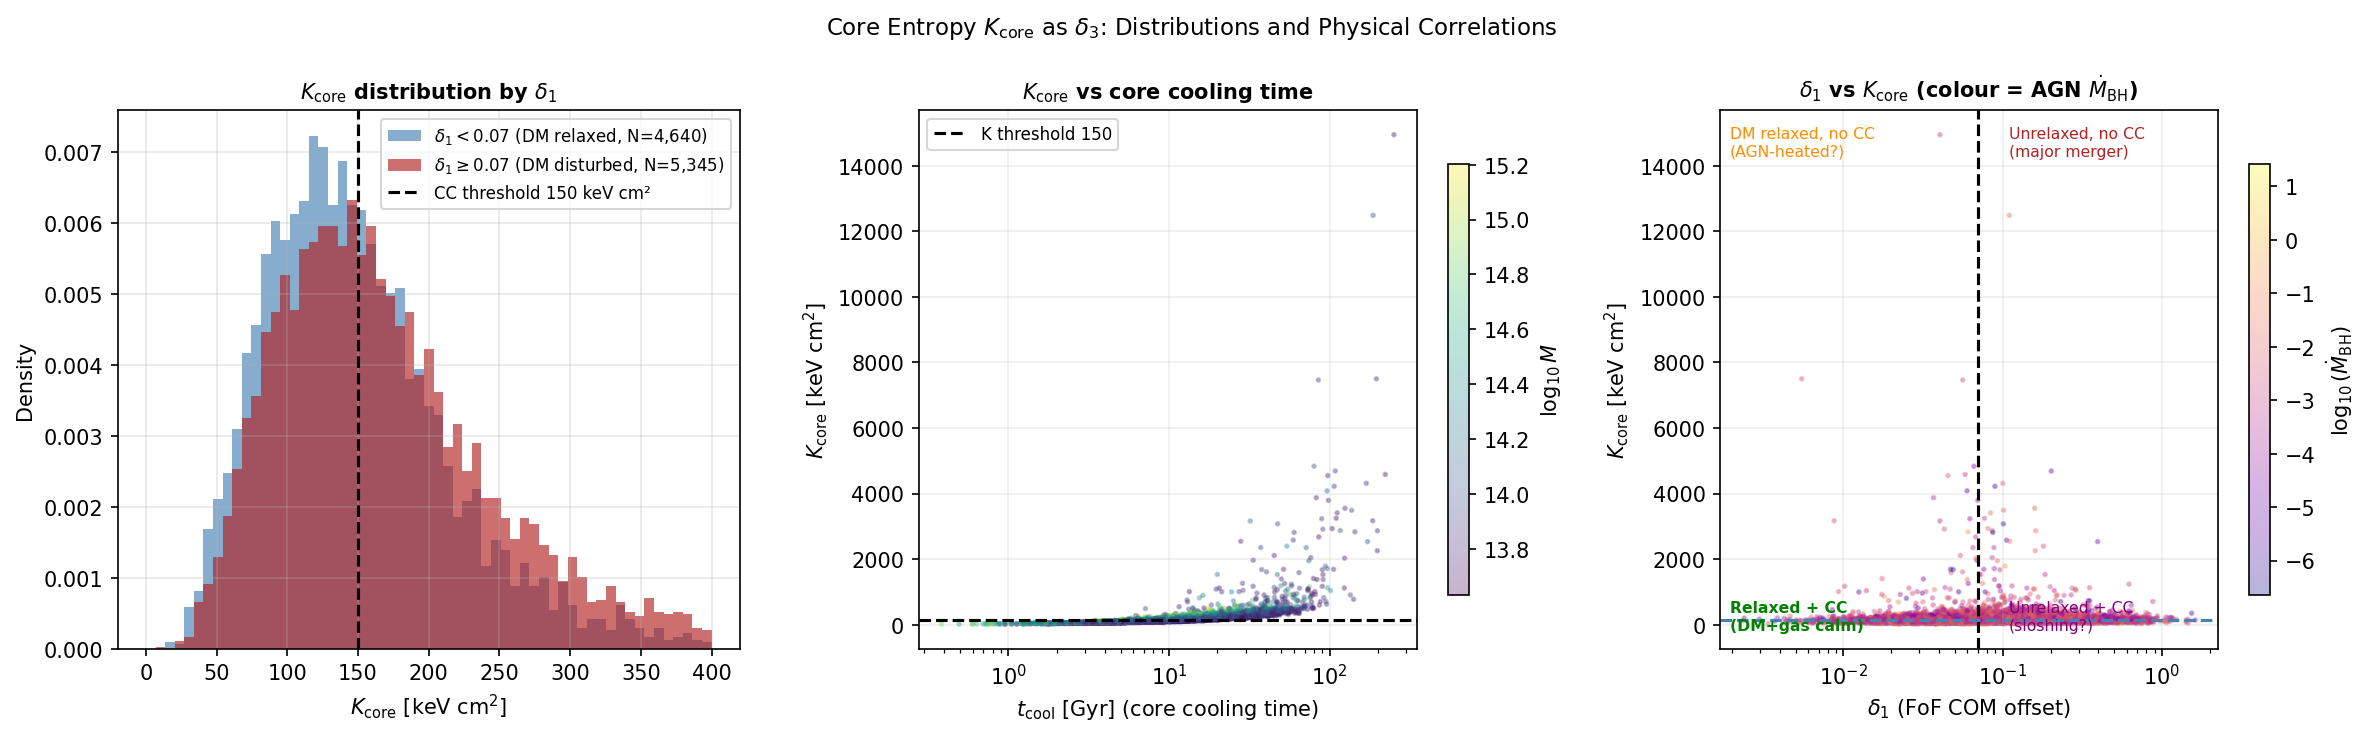
\includegraphics[width=\textwidth]{phase5_core_entropy_analysis.png}
  \caption{\textit{Left:} Distribution of $K_\mathrm{core}$ split by DM relaxation
  state ($\delta_1$). DM-relaxed halos (blue) are preferentially skewed toward
  lower core entropy (cool cores), but with substantial overlap --- confirming
  that $\delta_1$ and $\delta_3$ are complementary rather than redundant.
  \textit{Centre:} $K_\mathrm{core}$ vs.\ core cooling time $t_\mathrm{cool}$
  from the catalogue. The two are tightly correlated as expected from the
  definition of entropy, validating that the catalogue core entropy is physically
  meaningful and consistent with the cooling timescale.
  \textit{Right:} $\delta_1$ vs.\ $K_\mathrm{core}$ coloured by AGN black-hole
  accretion rate $\dot{M}_\mathrm{BH}$. The DM-relaxed/high-$K_\mathrm{core}$
  quadrant (AGN-heated category, orange in prior figures) shows elevated BHR,
  directly connecting the absence of a cool core to ongoing AGN feedback.
  The DM-disturbed/low-$K_\mathrm{core}$ quadrant (sloshing, purple) shows
  lower AGN activity, consistent with the cool core surviving the gravitational
  perturbation.}
  \label{fig:phase5_kcore}
\end{figure}

\subsection{Summary: What Each Criterion Probes}

\begin{center}
\begin{tabular}{p{2.2cm}p{4.5cm}p{4.5cm}p{2.8cm}}
\toprule
Criterion & Physical Process Probed & Timescale Probed & Observational Proxy \\
\midrule
$\delta_1$ (COM offset) &
  Coherent DM displacement from potential min; major mergers, pericentric passages &
  Short ($\lesssim\!1$ Gyr after merger) &
  Hard to observe directly; X-ray centroid shift \\
$\delta_2$ (DM--gas separation) &
  DM--gas decoupling; gas sloshing, ram pressure stripping, minor mergers &
  Intermediate (sloshing persists 1--5 Gyr) &
  X-ray morphology, offset from SZ centroid \\
$\delta_3$ (core entropy) &
  Core gas thermodynamics; cumulative cooling/heating history &
  Long (cool core builds over $\gtrsim\!2$ Gyr) &
  X-ray spectroscopy in core; accessible to Chandra, XMM, eROSITA \\
\bottomrule
\end{tabular}
\end{center}

%% ============================================================
\section{Phase 6: Nuanced $\delta_4$ and Comprehensive Stacked Profile Analysis}
\label{sec:phase6}

\begin{querybox}
\textcolor{red!80!black}{%
Add a nuanced $\delta_4$ combining direct catalog observables, closely related to profile
differences we expect to see. Expand the stacked profile analysis with DM relaxation
($\delta_1$) as the baseline for all, then show stacked profiles for DM-relaxed halos
split by each secondary criterion. Demonstrate profile differences at different radii
and their astrophysical implications.}
\end{querybox}

\subsection{The Fourth Criterion: Thermal Profile Indicator ($\delta_4$ = TPI)}

While $\delta_3 = K_\mathrm{core}$ encodes the combined effect of temperature and
density at the core, a more nuanced view separates these two independent observables:

\begin{equation}
  \delta_4 = \mathrm{TPI} = z(\ln n_{e,\mathrm{core}}) + z(\ln T_\mathrm{ratio}),
\end{equation}

where $z(\cdot)$ denotes a robust z-score (median/MAD normalisation), and:
\begin{itemize}
  \item $n_{e,\mathrm{core}}$ (\texttt{sod\_halo\_core\_ne}): core electron density ---
        a proxy for the \emph{amplitude} of the central density peak.
        Observable via X-ray surface brightness fitting.
  \item $T_\mathrm{ratio} = T_{500c}^\mathrm{BoloEx} / T_{500c}$: ratio of core-excised
        to total bolometric temperature.
        This measures the \emph{temperature drop} in the core ---
        high values ($> 1$) indicate the core is cooler than the cluster average,
        the classical cool-core spectroscopic signature.
        Observable from X-ray spectra with and without core excision.
\end{itemize}

\noindent $T_\mathrm{ratio}$ spans $[1.04, 1.09, 1.14, 1.18, 1.27]$ at the
[5, 25, 50, 75, 95] percentiles: the cool-core temperature suppression is detectable
but moderate in Frontier-E, consistent with the AGN feedback prescription.

\paragraph{Why TPI is more nuanced than $K_\mathrm{core}$.}
$K_\mathrm{core} = T_\mathrm{core} \times n_e^{-2/3}$ combines temperature and density
in a fixed ratio. TPI keeps $n_{e,\mathrm{core}}$ and $T_\mathrm{ratio}$ \emph{separate}.
The discordant cases are physically interesting:
\begin{itemize}
  \item \textbf{K-cool-core but low TPI} (14\% of valid halos):
        low $K_\mathrm{core}$ is achieved via moderate $n_e$ and moderate $T$ together,
        not through a strong density peak with a temperature drop. These halos would
        appear as ``cool-core'' in entropy but lack a spectroscopically detectable
        temperature gradient.
  \item \textbf{High TPI but non-CC by entropy} (17.5\%):
        elevated $n_{e,\mathrm{core}}$ \emph{and} clear $T_\mathrm{ratio}$ signature, but
        $K_\mathrm{core} > 150$ keV cm$^2$ --- possibly shock-heated dense cores or
        AGN-heated systems where the density peak persists but the entropy has risen.
\end{itemize}

We classify $R_4 = \mathrm{TPI} > 0$ (above-median combined score), giving
$5{,}344 / 9{,}985 = 53.5\%$ of valid halos as cool-core by TPI.

\subsection{Comprehensive Stacked Profile Comparison}

Figure~\ref{fig:phase6_stacked} presents the central result of this phase:
a $5 \times 4$ grid showing stacked median radial profiles with DM relaxation
as the universal baseline.

\begin{figure}[htbp]
  \centering
  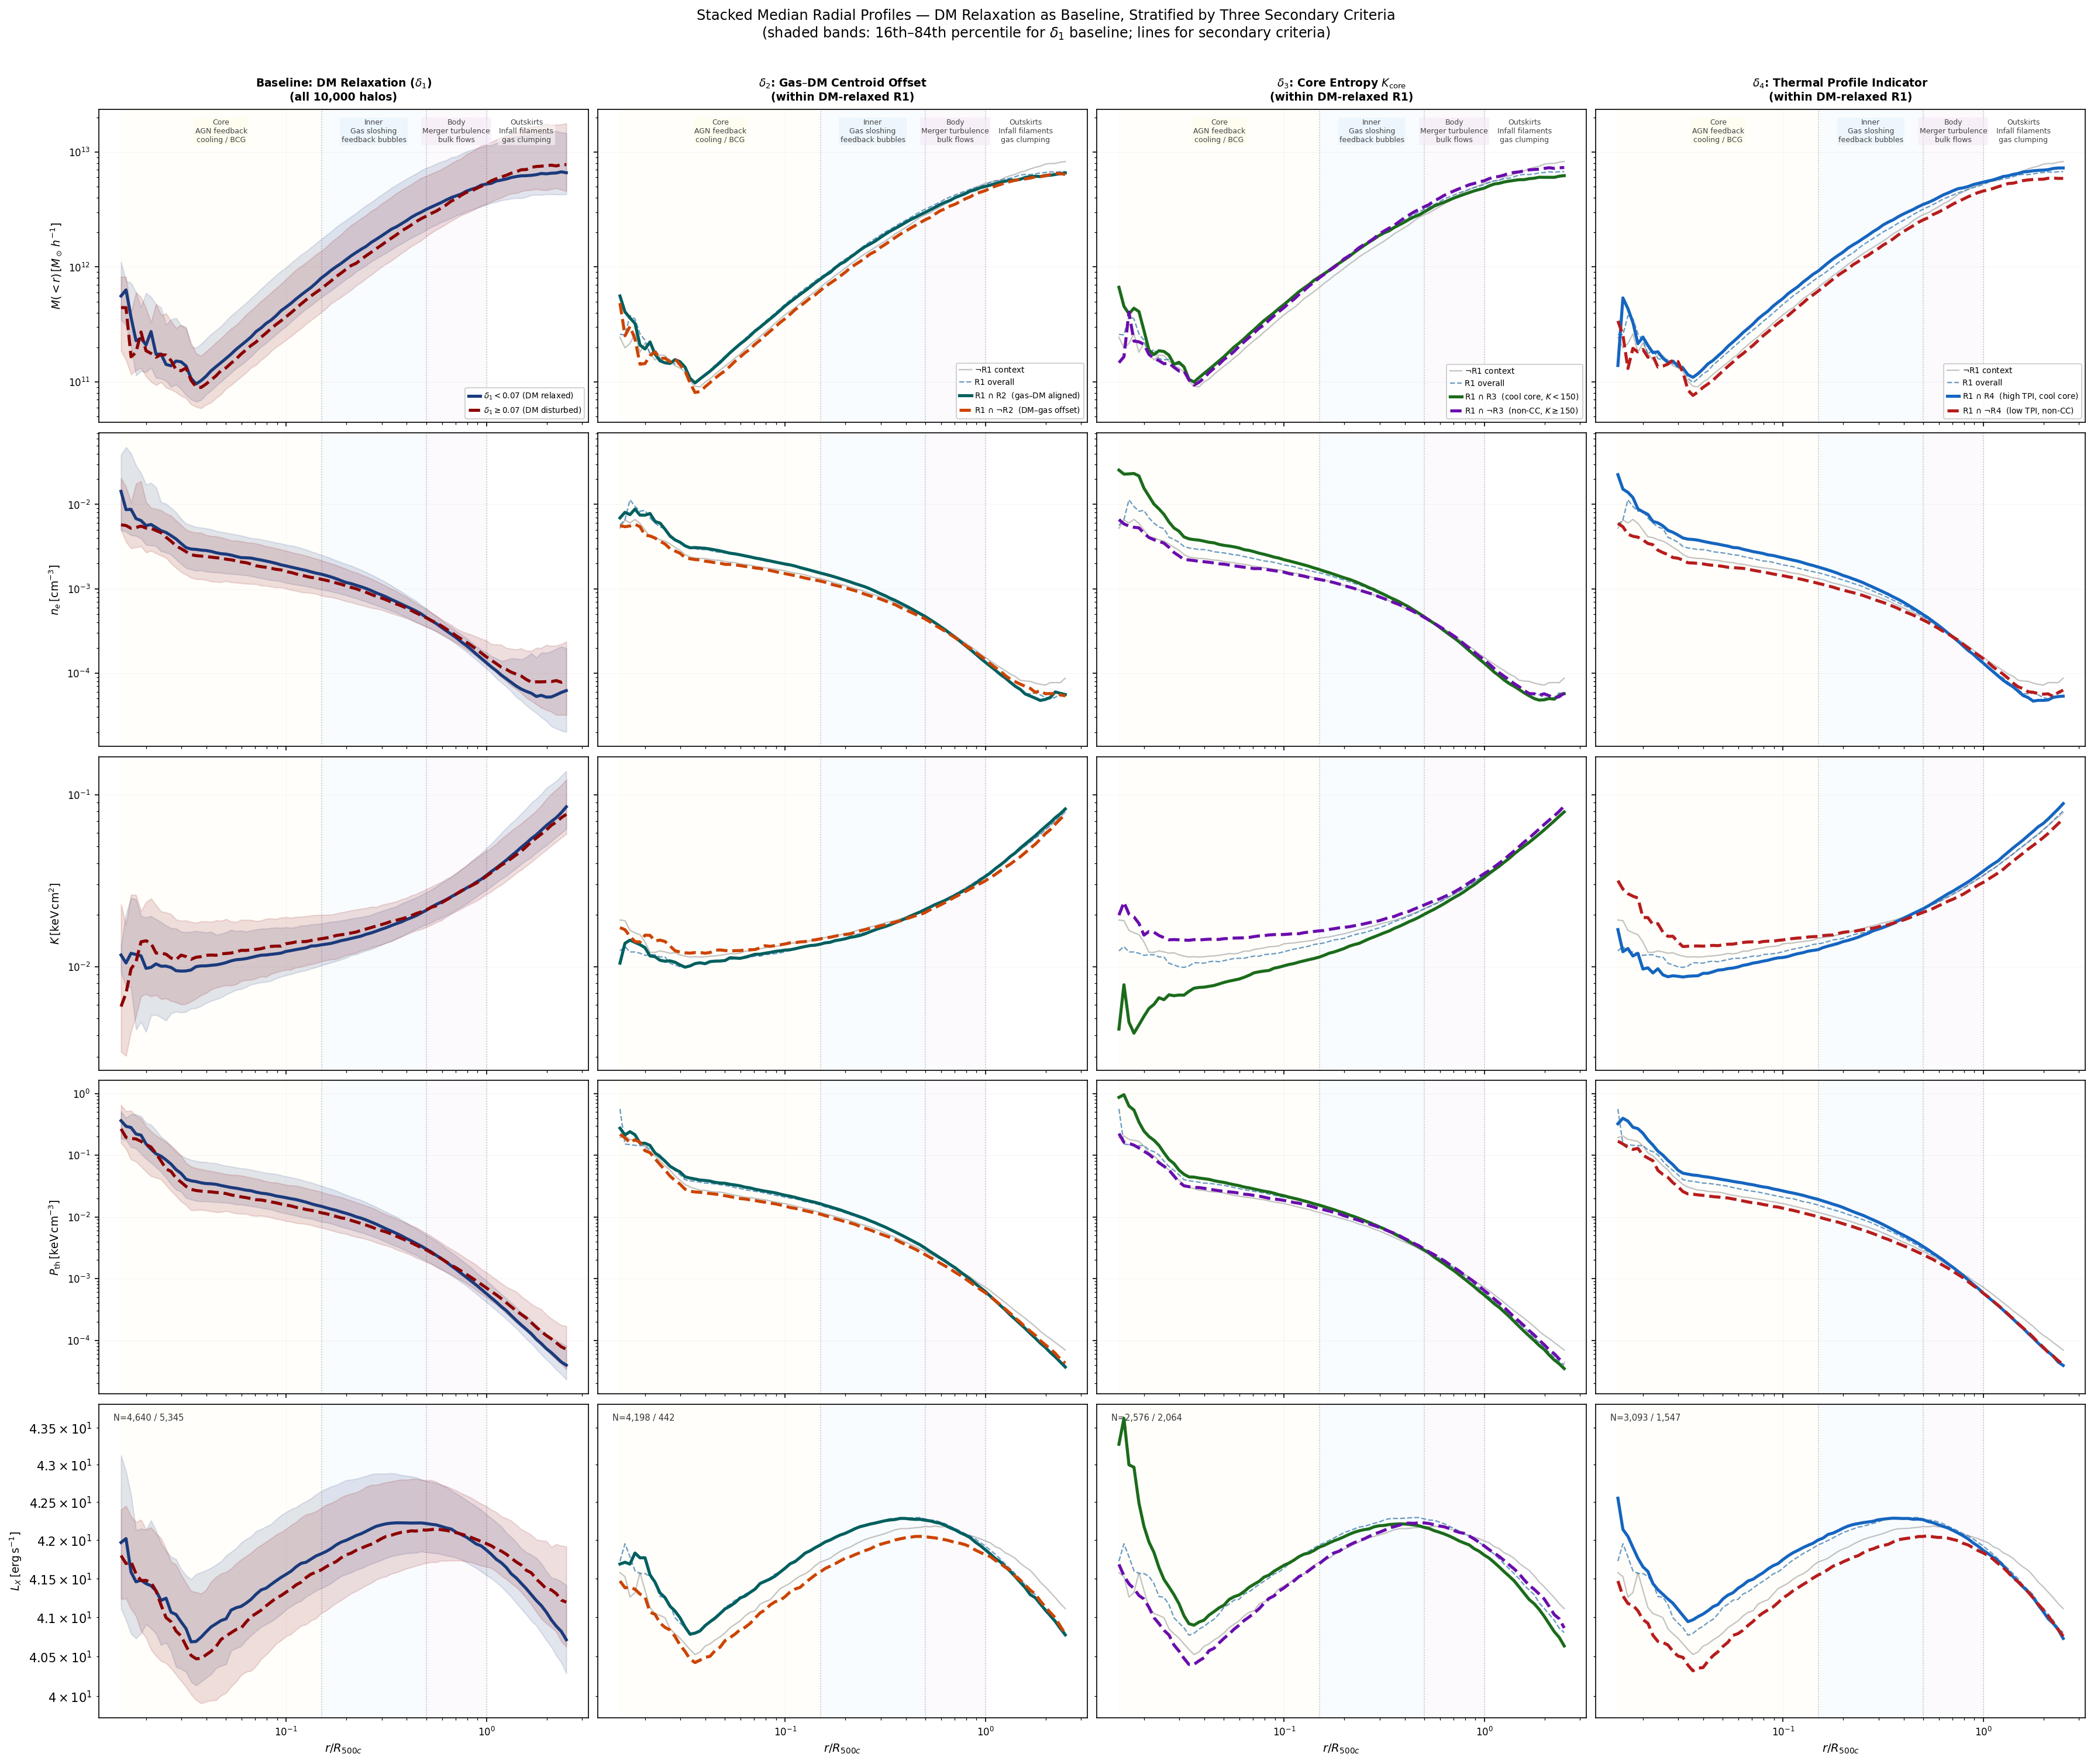
\includegraphics[width=\textwidth]{phase6_stacked_profiles_comprehensive.png}
  \caption{%
  Stacked median radial profiles for five observables (rows: enclosed mass, gas
  electron density, entropy, thermal pressure, X-ray luminosity) and four criteria
  (columns).
  \textbf{Column~0 (Baseline $\delta_1$):} All 10,000 halos split into DM-relaxed
  R1 (dark blue, with 16th--84th percentile bands) and DM-disturbed $\neg$R1 (dark red).
  The subsequent columns show only halos within the DM-relaxed R1 population, using
  the same $\neg$R1 and R1 lines (thin gray / thin dashed navy) as context.
  \textbf{Column~1 ($\delta_2$: Gas--DM alignment):} Within R1, halos with aligned
  DM and gas centroids (R1$\cap$R2, teal) vs.\ those with a significant offset
  (R1$\cap\neg$R2, orange-red).
  \textbf{Column~2 ($\delta_3$: Core entropy):} R1$\cap$R3 (cool-core, green)
  vs.\ R1$\cap\neg$R3 (non-cool-core, purple).
  \textbf{Column~3 ($\delta_4$: TPI):} R1$\cap$R4 (high TPI, blue) vs.\
  R1$\cap\neg$R4 (low TPI, red).
  Shaded background zones mark four astrophysical regimes (yellow: core $r<0.15\,R_{500c}$;
  blue: inner $0.15$--$0.5\,R_{500c}$; purple: body $0.5$--$1\,R_{500c}$; white: outskirts).}
  \label{fig:phase6_stacked}
\end{figure}

\paragraph{Key physics, column by column.}

\begin{description}
  \item[$\delta_1$ baseline (column 0):]
    The $n_e$ and entropy profiles show the broadest separation between R1 and $\neg$R1.
    DM-relaxed halos (R1) have on average lower entropy and higher central $n_e$,
    confirming that DM relaxation correlates with core cooling.
    The mass profiles are nearly identical, confirming that the mass split
    is not the driver.
    L$_X$ shows elevated R1 emission at $r < 0.5\,R_{500c}$, with $\neg$R1 catching
    up at intermediate radii (more extended emission in disturbed systems).

  \item[$\delta_2$: Gas--DM alignment (column 1):]
    Within R1, the profile differences between R1$\cap$R2 and R1$\cap\neg$R2 are
    concentrated at \emph{intermediate radii} ($0.15$--$0.7\,R_{500c}$).
    The R1$\cap\neg$R2 halos (gas offset from DM) show elevated entropy and pressure
    at $0.3$--$0.6\,R_{500c}$ --- the fingerprint of gas sloshing: an off-axis perturbation
    has displaced the gas, creating a contact discontinuity (cold front) between the
    cooler displaced gas and the ambient ICM.
    The core ($r < 0.15\,R_{500c}$) is nearly indistinguishable --- confirming that
    sloshing moves gas at intermediate radii while leaving the core itself intact.
    This is a hallmark of the observationally well-known sloshing cluster morphology.

  \item[$\delta_3$: Core entropy (column 2):]
    The largest profile differences of all four columns appear here, concentrated
    entirely in the \emph{core} ($r < 0.15\,R_{500c}$):
    R1$\cap$R3 halos show $n_e$ enhanced by $>10\times$ and L$_X$ enhanced by
    $>100\times$ at $r < 0.05\,R_{500c}$ compared to R1$\cap\neg$R3.
    Outside $0.3\,R_{500c}$, profiles converge --- the core entropy criterion
    is essentially blind to the outer cluster environment.
    This is exactly the expected signature of radiative cooling: gas condenses
    in the centre over Gyr timescales, boosting $n_e$ and $L_X$ while leaving
    the outer DM potential and gas distribution unchanged.

  \item[$\delta_4$: TPI (column 3):]
    TPI reproduces the core-dominated separation of $\delta_3$ but with an additional
    element: halos with R1$\cap\neg$R4 (low TPI) show a broader suppression of
    $n_e$ extending to $0.3\,R_{500c}$ that is not seen in R1$\cap\neg$R3.
    This indicates that TPI is sensitive to the \emph{slope} of the density profile
    as well as the peak: halos with a high core density but a steep outward drop
    (classic cool-core) score high, while halos with a moderate density that drops
    more gradually (possibly post-heating remnant cores) score lower than K alone
    would suggest.
    The T$_\mathrm{ratio}$ component also contributes at intermediate radii through
    the global temperature measurement, extending the discriminating power slightly
    beyond the innermost bin.
\end{description}

\subsection{Profile Ratio Maps: Radial Discrimination Power}

Figure~\ref{fig:phase6_ratio} quantifies where in radius each criterion is most
discriminating, using $\log_{10}[\mathrm{median}(R1\cap R_x) / \mathrm{median}(R1\cap\neg R_x)]$.

\begin{figure}[htbp]
  \centering
  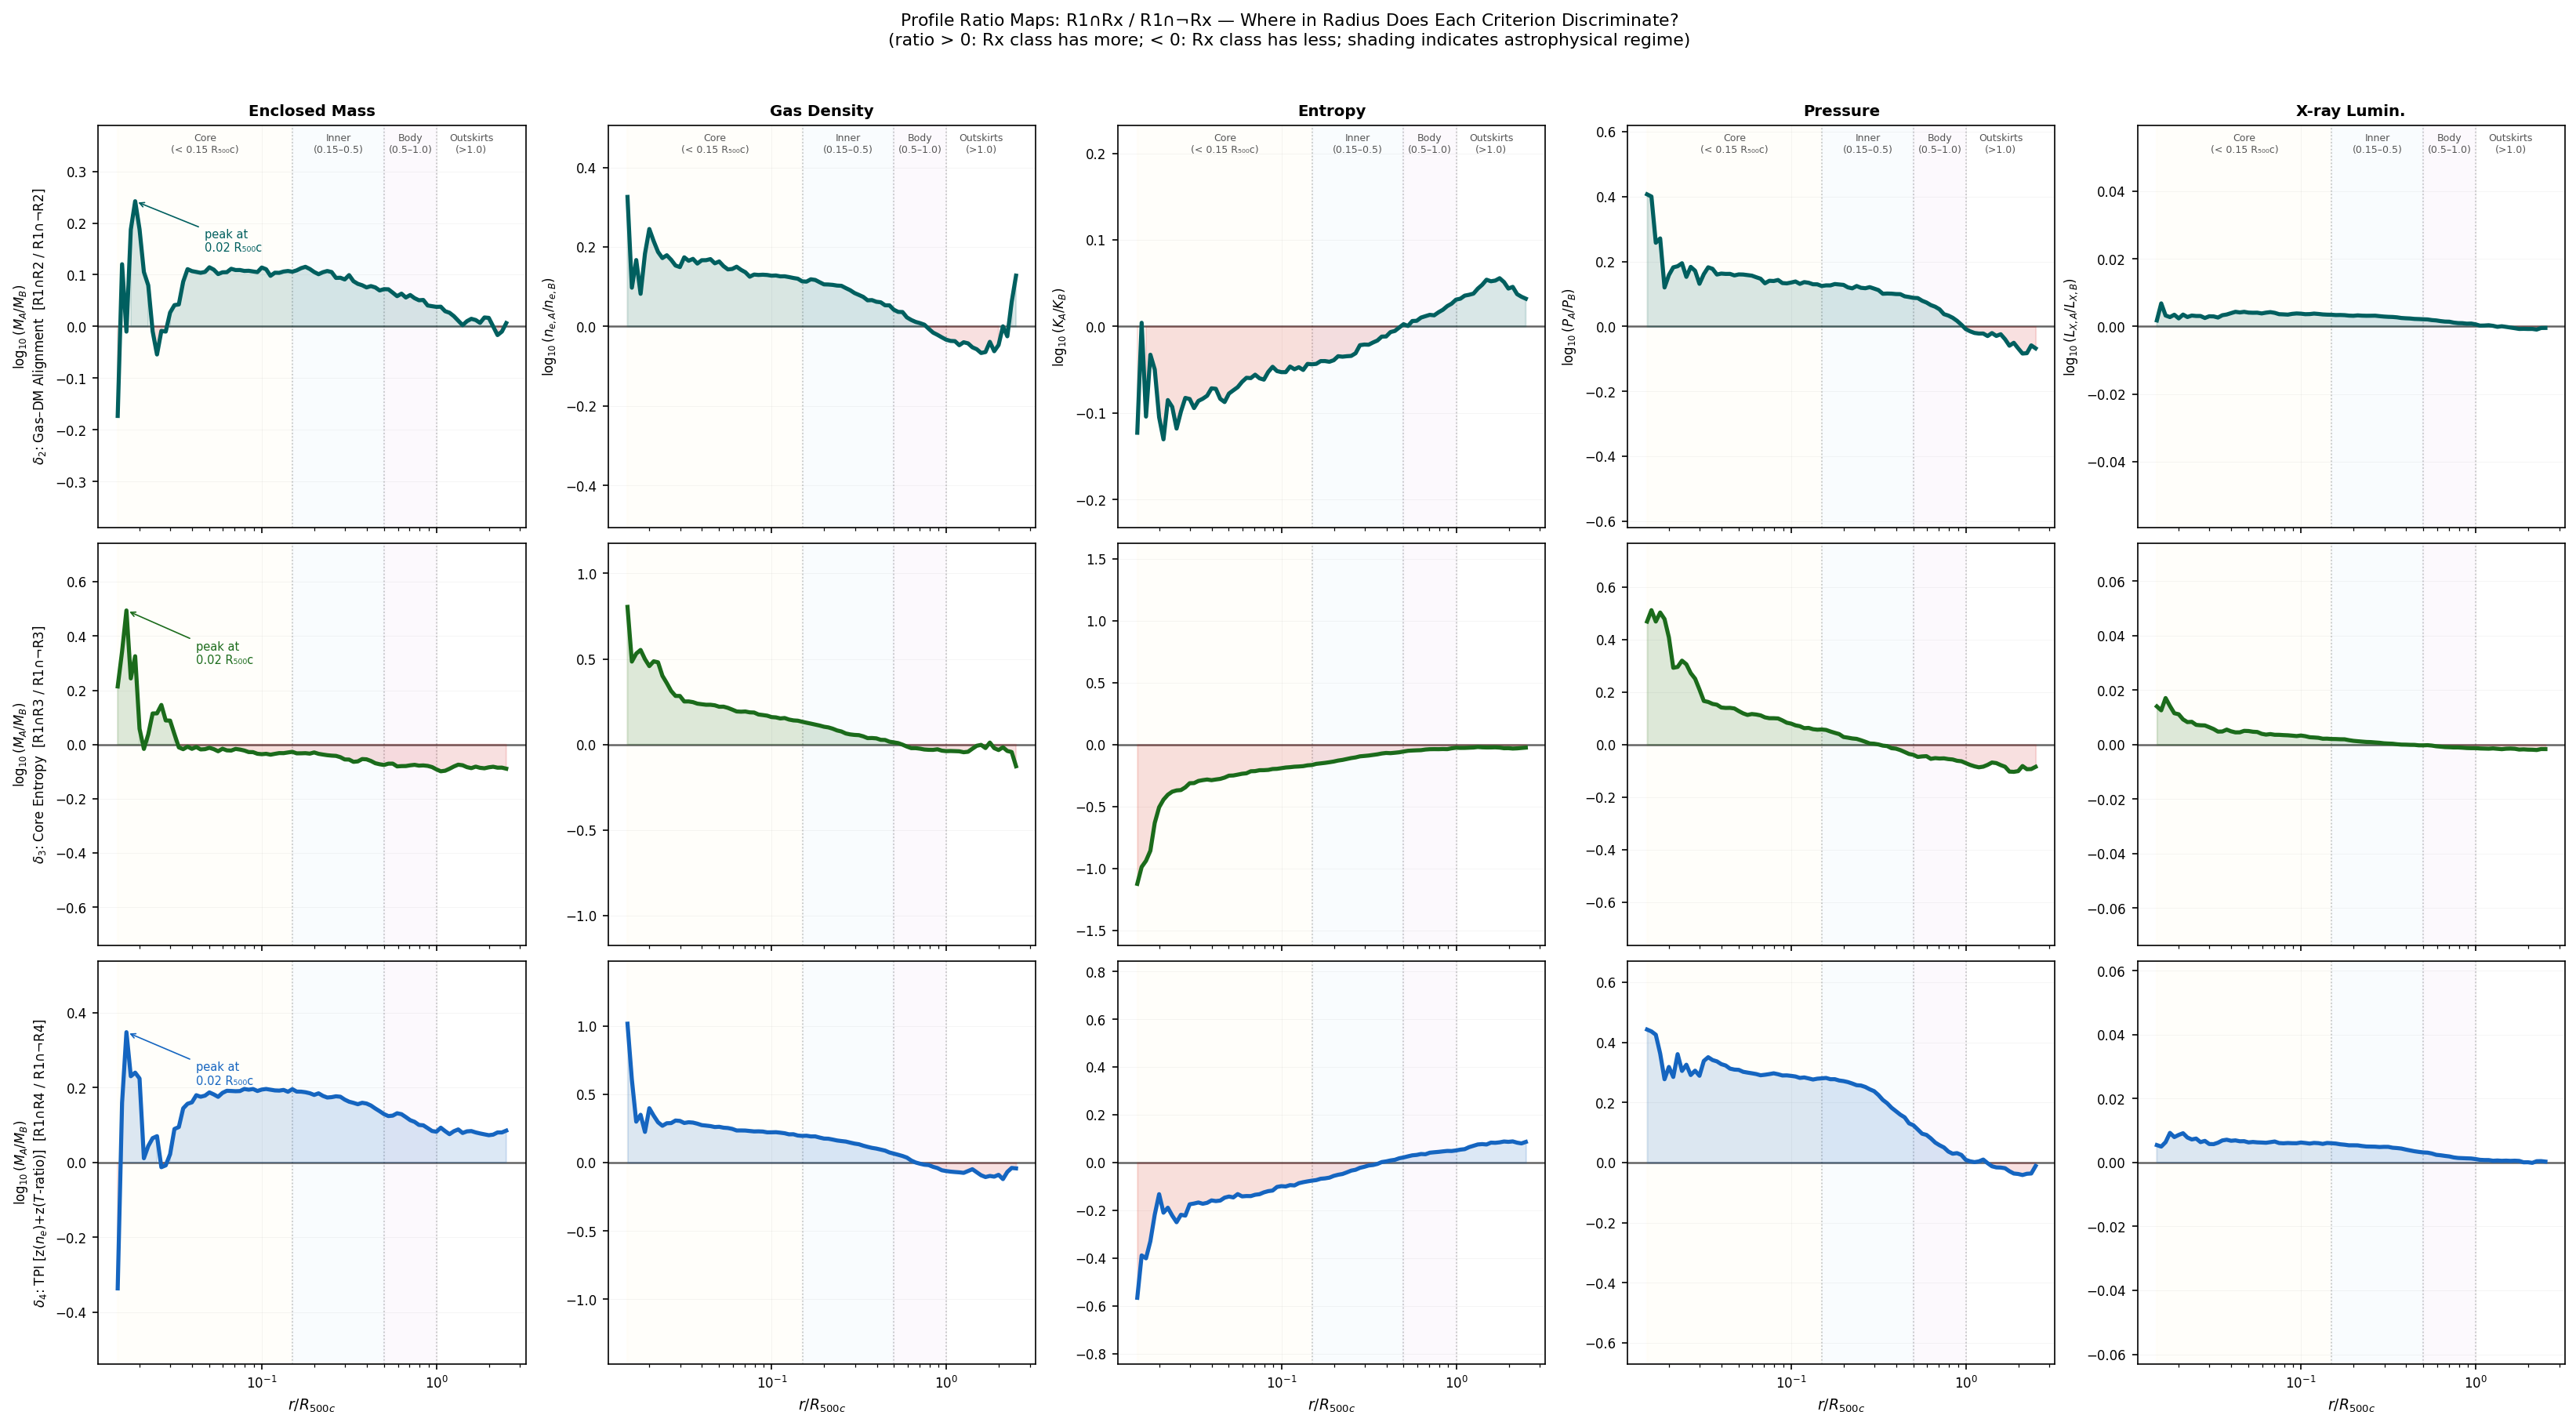
\includegraphics[width=\textwidth]{phase6_ratio_profiles.png}
  \caption{%
  Log-ratio of stacked profiles between ``relaxed'' and ``unrelaxed'' sub-populations
  within DM-relaxed halos, for each secondary criterion (rows) and each profile type
  (columns).
  Positive values (solid-filled): the Rx class has more of this quantity.
  Negative values (red-filled): the Rx class has less.
  The horizontal line marks ratio~=~1; vertical dotted lines mark 0.15, 0.5,
  and $1.0\,R_{500c}$.
  \textbf{Key result:}
  $\delta_2$ (gas--DM alignment) peaks in the ratio at $0.3$--$0.7\,R_{500c}$ for
  entropy and pressure --- the sloshing cold-front regime.
  $\delta_3$ and $\delta_4$ peak strongly at $r < 0.1\,R_{500c}$ for $n_e$ and $L_X$,
  and remain elevated to $\sim 0.3\,R_{500c}$.
  $\delta_4$ (TPI) shows a slightly wider ratio profile than $\delta_3$ in $n_e$
  and pressure, reflecting the sensitivity to the density slope captured
  by the T$_\mathrm{ratio}$ component.}
  \label{fig:phase6_ratio}
\end{figure}

\subsection{TPI Diagnostic: Where $\delta_3$ and $\delta_4$ Disagree}

Figure~\ref{fig:phase6_tpi} shows the TPI component space and the concordance
between $\delta_3$ and $\delta_4$.

\begin{figure}[htbp]
  \centering
  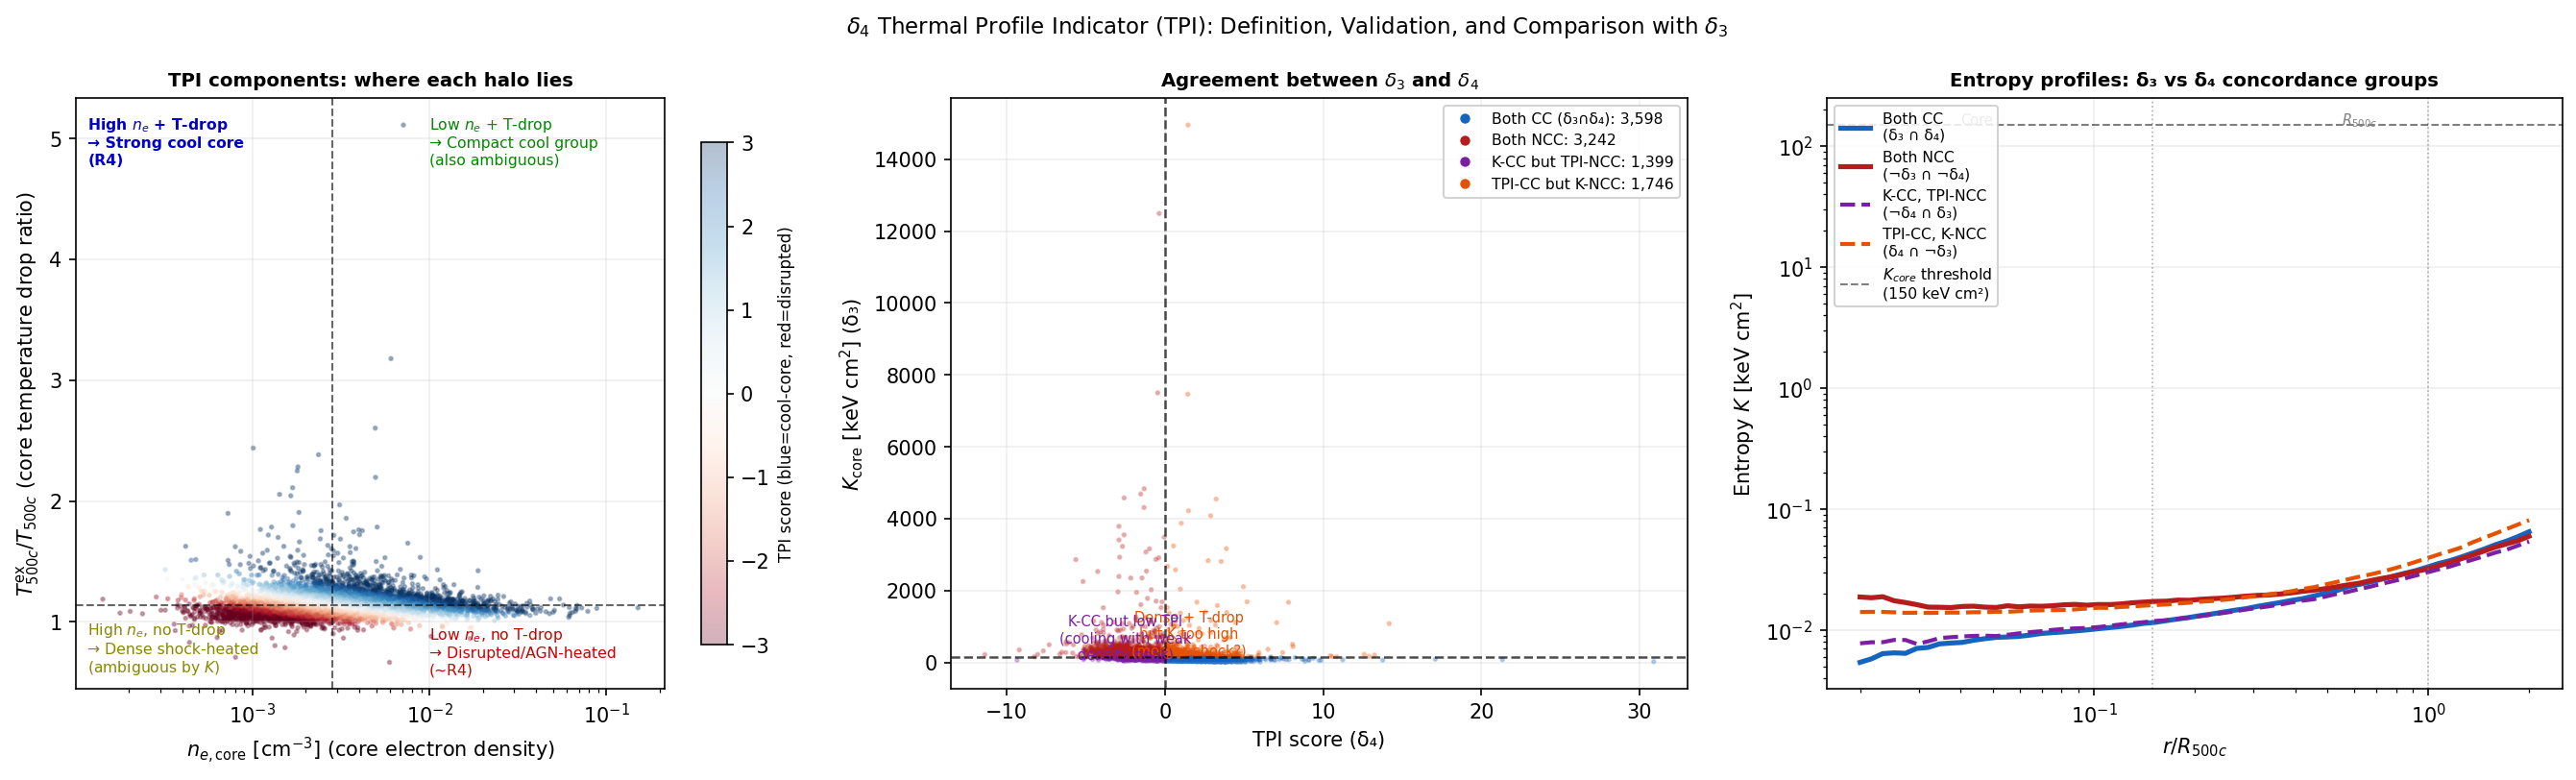
\includegraphics[width=\textwidth]{phase6_tpi_diagnostic.png}
  \caption{%
  \textit{Left:} Core electron density $n_{e,\mathrm{core}}$ vs.\ temperature
  ratio $T_{500c}^\mathrm{BoloEx}/T_{500c}$, coloured by TPI score (blue~=~high TPI,
  i.e.\ cool-core; red~=~low TPI). The quadrant structure identifies four physically
  distinct regimes annotated in the panel.
  \textit{Centre:} TPI ($\delta_4$) vs.\ $K_\mathrm{core}$ ($\delta_3$) for all
  valid halos, coloured by the $\delta_3$/$\delta_4$ agreement state.
  The $3{,}598$ halos where both criteria agree on cool-core (blue) form a tight
  sequence; the $1{,}746$ TPI-cool-core / K-non-CC halos (orange) lie at high TPI
  but moderate $K_\mathrm{core}$, consistent with dense, high-T cores.
  \textit{Right:} Stacked entropy profiles for the four concordance groups, revealing
  that the K-CC/TPI-CC (blue) group has the steepest entropy gradient, while the
  discordant groups occupy intermediate positions.
  }
  \label{fig:phase6_tpi}
\end{figure}

\subsection{Summary: Criterion--Profile--Radius Map}

Table~\ref{tab:profile_radius} summarises which criterion discriminates most strongly,
at which radius, and in which observable.

\begin{table}[htbp]
\centering
\caption{Primary radial regime and dominant observable for each relaxation criterion.}
\label{tab:profile_radius}
\begin{tabular}{llll}
\toprule
Criterion & Dominant radius & Most discriminating profile & Physical driver \\
\midrule
$\delta_1$ (FoF COM) & $0.3$--$2\,R_{500c}$ & Entropy, $L_X$ & Major merger \& DM bulk motion \\
$\delta_2$ (DM--gas centroid) & $0.2$--$0.7\,R_{500c}$ & Entropy, Pressure & Gas sloshing cold fronts \\
$\delta_3$ (core entropy) & $r < 0.15\,R_{500c}$ & $n_e$, $L_X$ & Radiative cooling vs.\ AGN heating \\
$\delta_4$ (TPI) & $r < 0.3\,R_{500c}$ & $n_e$, $L_X$, Pressure & Density peak \emph{and} T-gradient \\
\bottomrule
\end{tabular}
\end{table}

%% ============================================================
\section{Phase 7: Particle Morphology Visualizations}
\label{sec:phase7}

\begin{querybox}
Visualize the shortlist halos using particle projections (dark matter, stars, gas, gas
temperature), organized by relaxation group.  Create a combined gallery figure showing the
most extreme halo per group side by side with the four fields.
\end{querybox}

\noindent
Particle projections provide direct visual access to the morphological differences that
the stacked profiles summarize statistically.  Figure~\ref{fig:gallery} presents the
rank-1 (most extreme) halo from each of the seven relaxation sub-classes in a single
panel, enabling direct visual comparison across all groups.

\begin{figure*}[htbp]
  \centering
  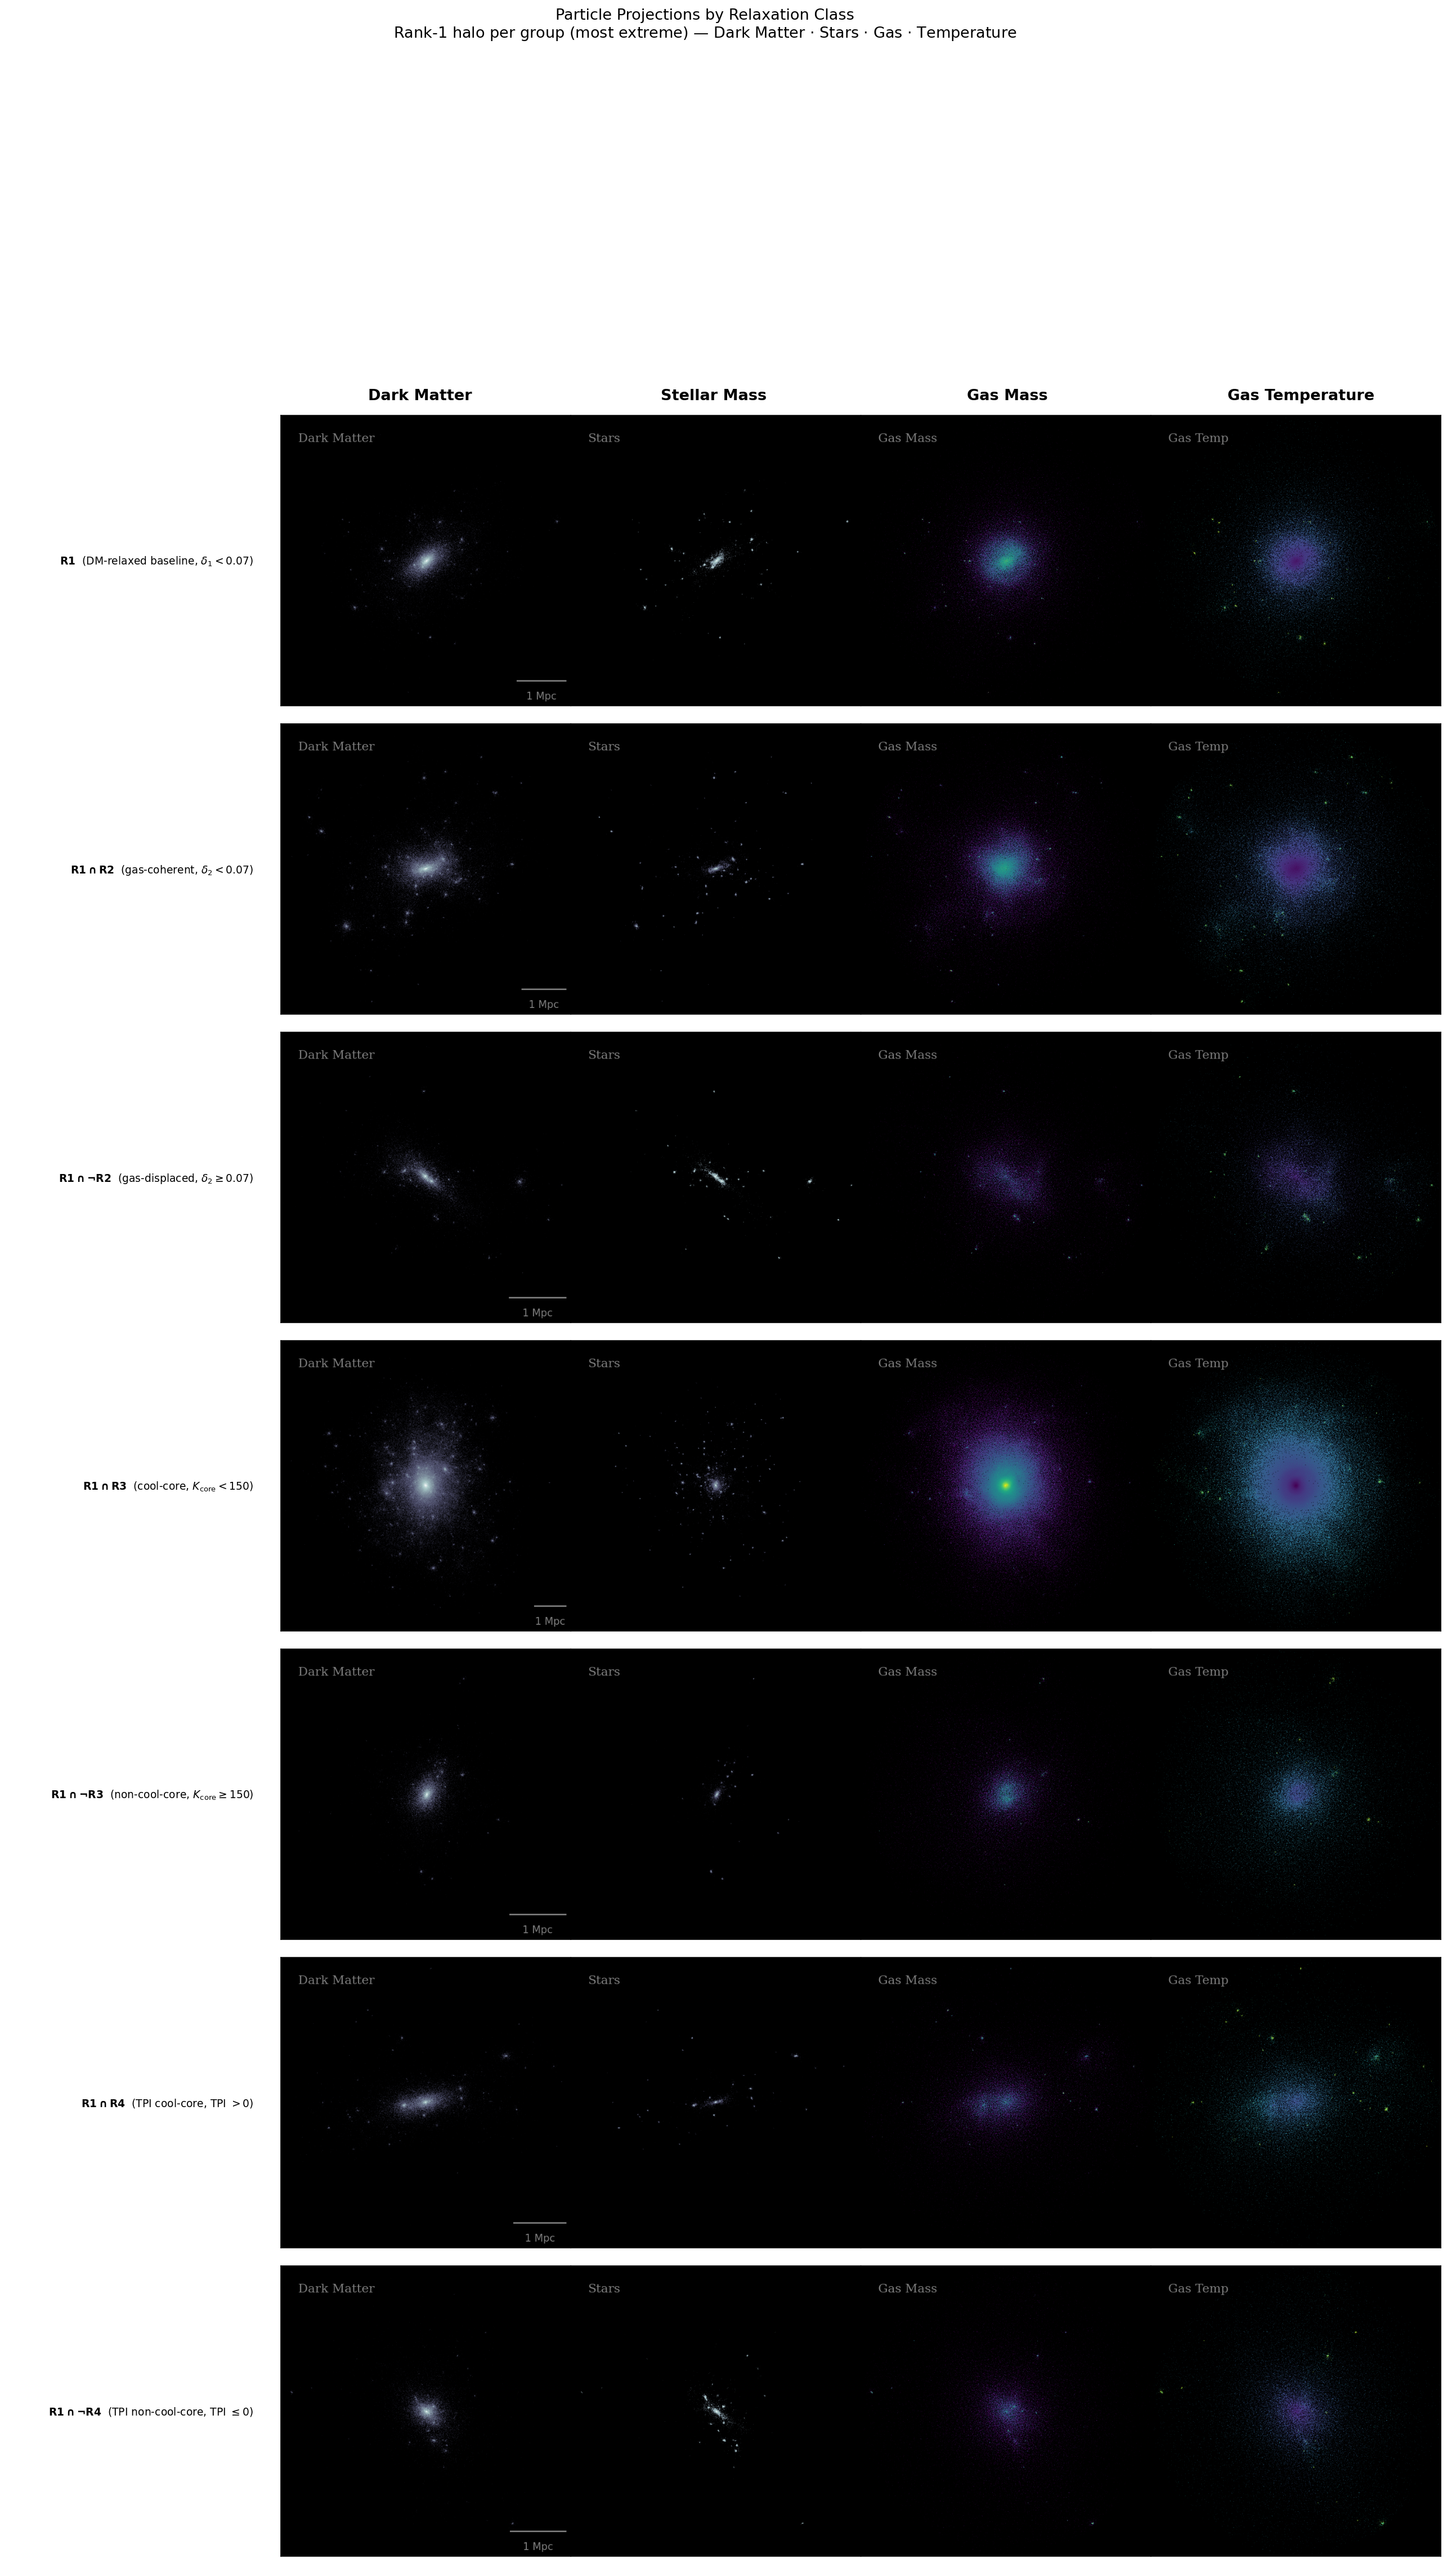
\includegraphics[width=\textwidth]{phase7_particle_gallery.png}
  \caption{Particle projection gallery --- rank-1 halo per group.  Each row shows the
    most extreme halo in one relaxation sub-class, rendered in four channels:
    dark matter mass (bone), stellar mass (bone), gas mass (viridis), and gas temperature
    (reversed viridis).  Group labels on the left identify the criterion and threshold.
    The qualitative contrasts visible here --- centred vs.\ offset gas in R1$\cap$R2 vs.\
    R1$\cap\lnot$R2, compact bright core vs.\ diffuse gas in R1$\cap$R3 vs.\
    R1$\cap\lnot$R3, temperature inversion vs.\ uniform warmth in R1$\cap$R4 vs.\
    R1$\cap\lnot$R4 --- mirror the stacked profile differences in
    Figures~\ref{fig:phase6_stacked} and~\ref{fig:phase6_ratio}.}
  \label{fig:gallery}
\end{figure*}

Figures~\ref{fig:mf_R1}--\ref{fig:mf_R1notR4} show six randomly selected halos from
each group, providing a broader view of morphological diversity within each sub-class.

\begin{figure*}[htbp]
  \centering
  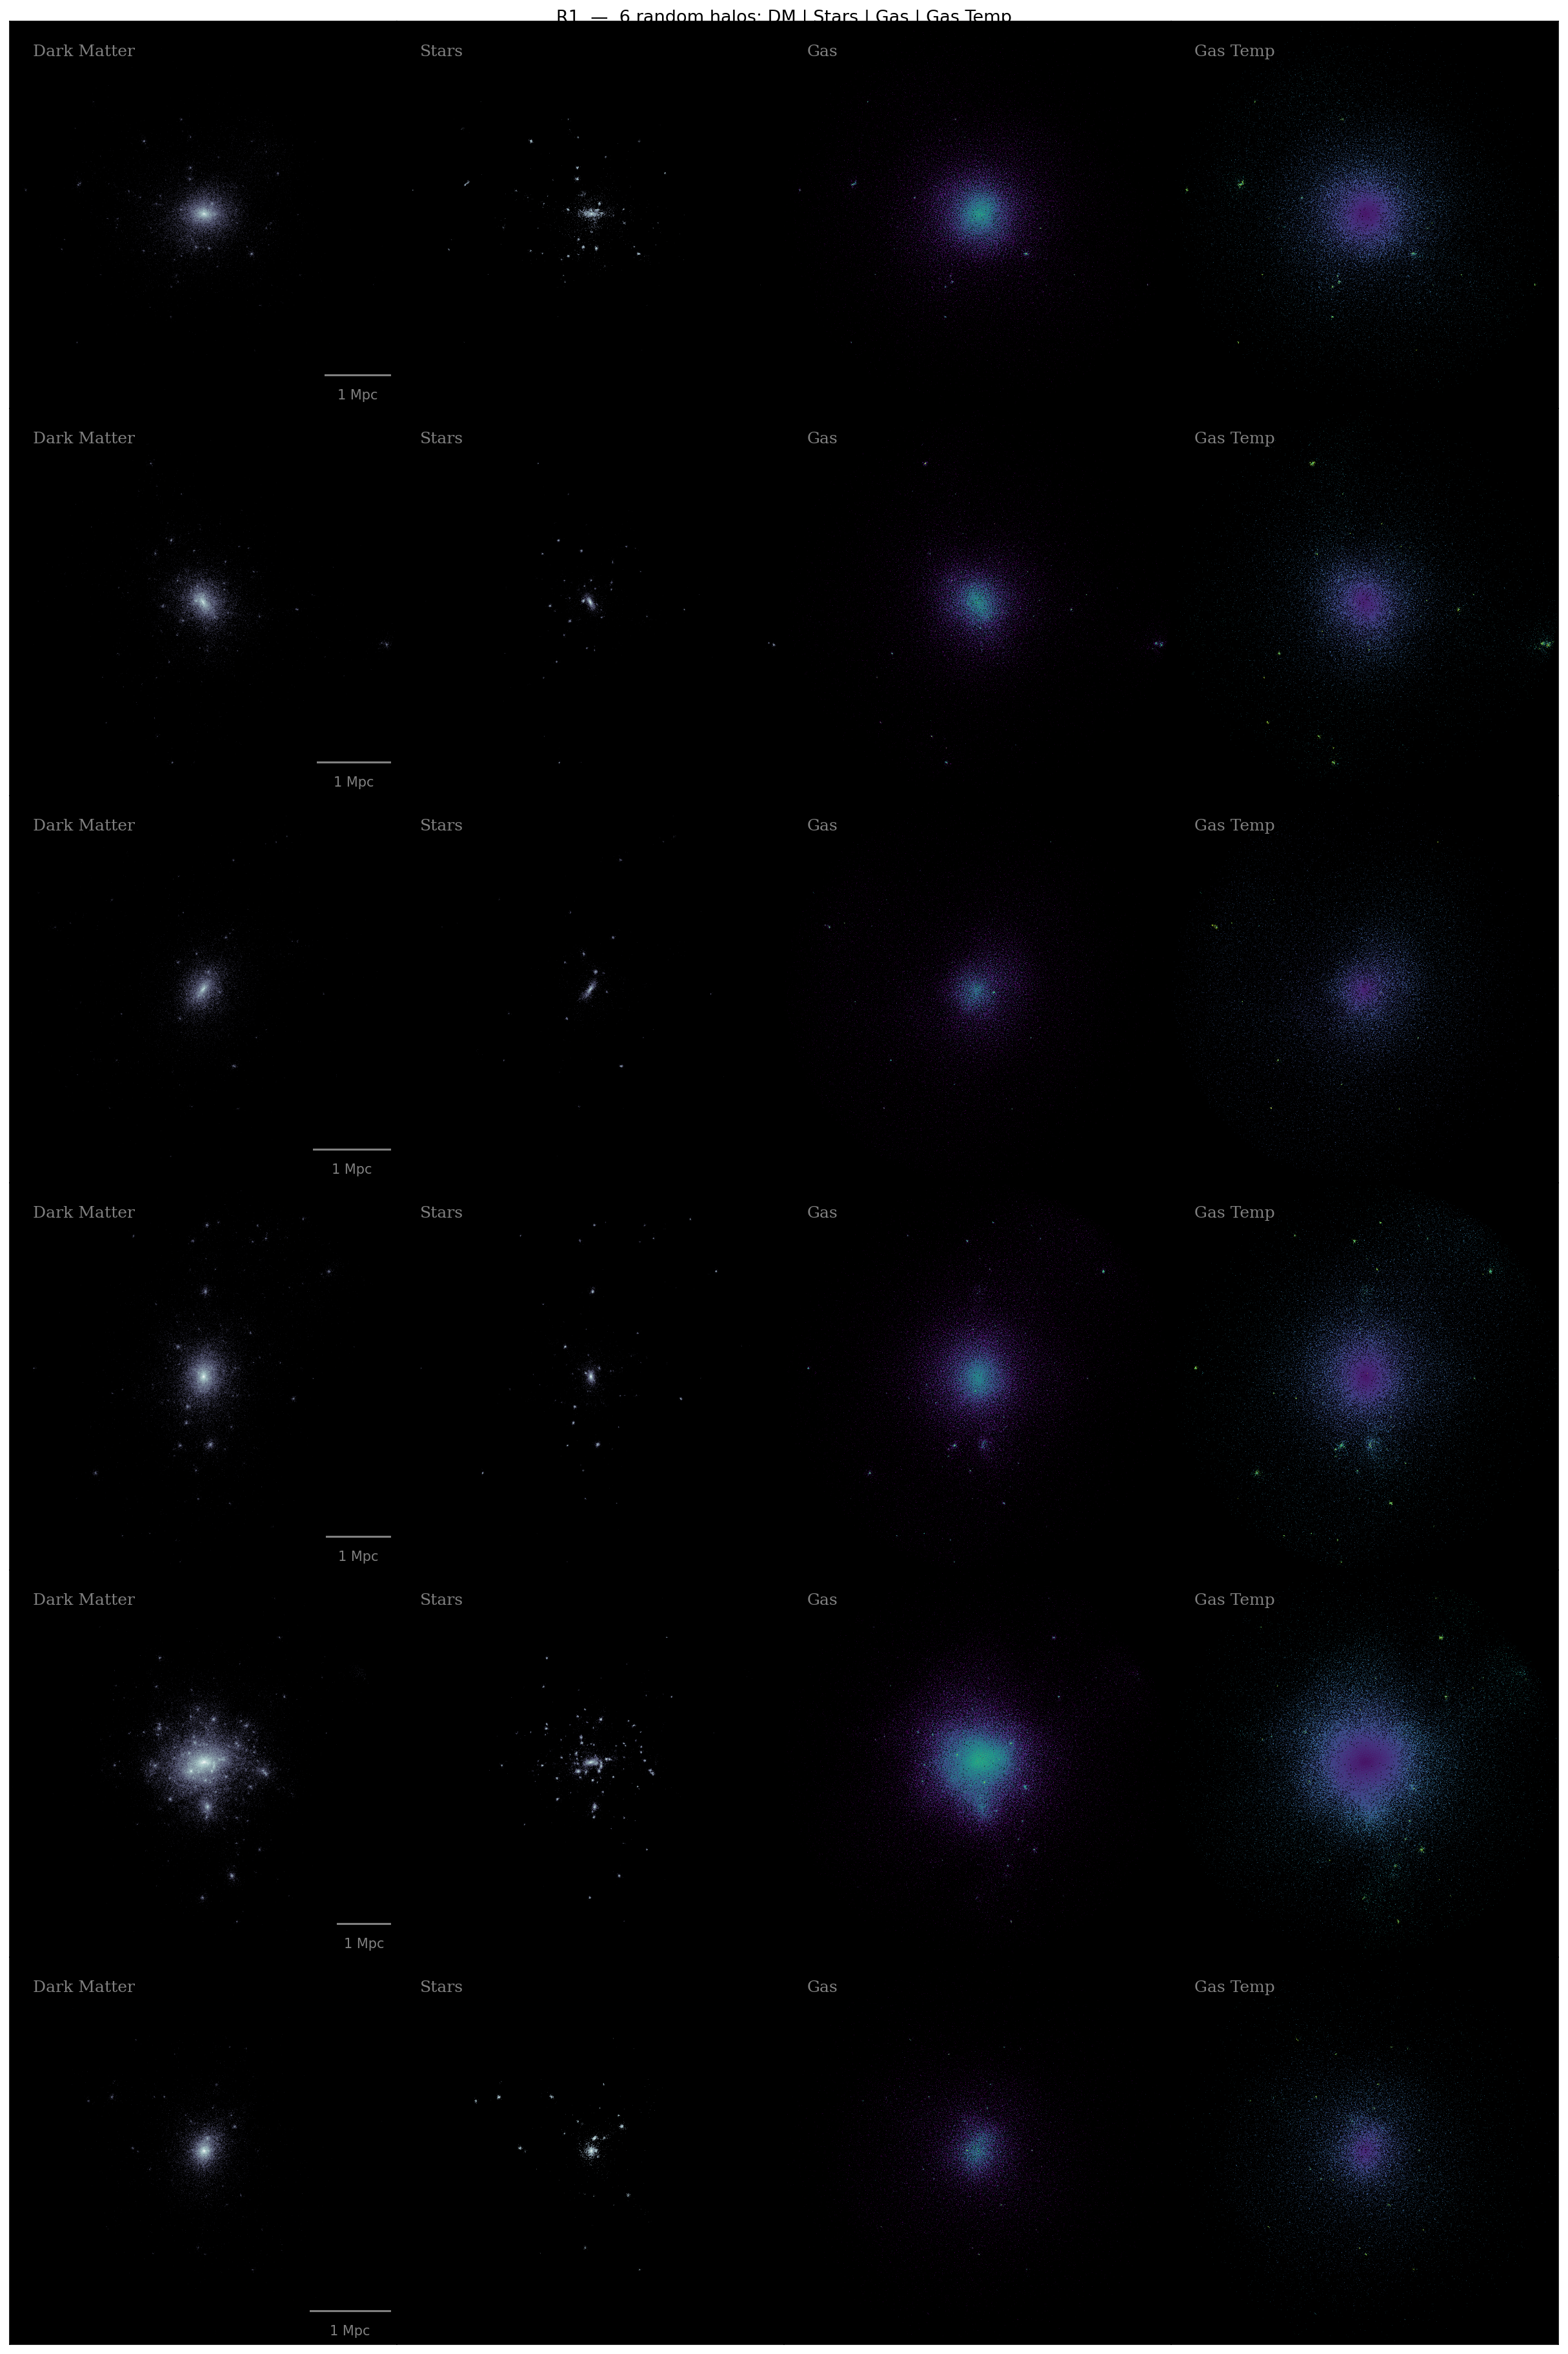
\includegraphics[width=\textwidth]{halo_viz/R1/multifield_4field_random6.png}
  \caption{Six randomly selected R1 halos (DM-relaxed baseline, $\delta_1 < 0.07$).
    Rows = halos; columns = dark matter, stars, gas mass, gas temperature.}
  \label{fig:mf_R1}
\end{figure*}

\begin{figure*}[htbp]
  \centering
  
\includegraphics[width=\textwidth]{halo_viz/R1_andR2/multifield_4field_random6.png}
  \caption{Six randomly selected R1$\cap$R2 halos (gas-coherent, $\delta_2 < 0.07$).
    Gas distributions closely trace the DM halo in all cases.}
  \label{fig:mf_R1andR2}
\end{figure*}

\begin{figure*}[htbp]
  \centering
  
\includegraphics[width=\textwidth]{halo_viz/R1_notR2/multifield_4field_random6.png}
  \caption{Six randomly selected R1$\cap\lnot$R2 halos (gas-displaced, $\delta_2 \geq 0.07$).
    Several examples show a clear offset between the DM centroid and the gas centroid.}
  \label{fig:mf_R1notR2}
\end{figure*}

\begin{figure*}[htbp]
  \centering
  
\includegraphics[width=\textwidth]{halo_viz/R1_andR3/multifield_4field_random6.png}
  \caption{Six randomly selected R1$\cap$R3 halos (cool-core, $K_\mathrm{core} < 150\,\mathrm{keV\,cm^2}$).
    Compact, centrally concentrated gas with blue temperature cores is characteristic.}
  \label{fig:mf_R1andR3}
\end{figure*}

\begin{figure*}[htbp]
  \centering
  
\includegraphics[width=\textwidth]{halo_viz/R1_notR3/multifield_4field_random6.png}
  \caption{Six randomly selected R1$\cap\lnot$R3 halos (non-cool-core,
    $K_\mathrm{core} \geq 150\,\mathrm{keV\,cm^2}$).  Gas cores are diffuse and
    isothermal.}
  \label{fig:mf_R1notR3}
\end{figure*}

\begin{figure*}[htbp]
  \centering
  
\includegraphics[width=\textwidth]{halo_viz/R1_andR4/multifield_4field_random6.png}
  \caption{Six randomly selected R1$\cap$R4 halos (TPI cool-core, TPI $> 0$).}
  \label{fig:mf_R1andR4}
\end{figure*}

\begin{figure*}[htbp]
  \centering
  
\includegraphics[width=\textwidth]{halo_viz/R1_notR4/multifield_4field_random6.png}
  \caption{Six randomly selected R1$\cap\lnot$R4 halos (TPI non-cool-core, TPI $\leq 0$).}
  \label{fig:mf_R1notR4}
\end{figure*}

%% ============================================================
\section{Summary and Outlook}
\label{sec:summary}

Six phases have been completed in this interactive research session:
\begin{itemize}
  \item \textbf{Phase 1}: Downloaded 10,000 Frontier-E halos with 51-bin radial profiles;
        visualised 10 profile types for a mass-stratified sample.
  \item \textbf{Phase 2}: Compared profiles to ideal references (NFW, Voit entropy baseline,
        Arnaud UPP), revealing central entropy bimodality and metallicity gradients.
  \item \textbf{Phase 3}: Directly fitted five models to the data; entropy slopes
        $n \approx 0.5$ (below the non-radiative 1.1) and higher total-density
        NFW concentrations in baryonically concentrated halos.
  \item \textbf{Phase 4}: Computed COM-offset metrics for all 10,000 halos. Entropy slope
        is the strongest correlate with $\delta_1$ ($\rho=-0.32$); $\delta_1$ and $\delta_2$
        only weakly correlated ($\rho=0.26$).
  \item \textbf{Phase 5}: Introduced $\delta_3 = K_\mathrm{core}$ (core entropy).
        Found that concordant relaxed halos (24\%) are the tightest scaling-relation
        subsample; sloshing cool-core halos (24\%) are the dominant source of
        $L_X$ scatter in X-ray surveys; AGN-heated halos (18\%) connect high core
        entropy to elevated BHR; total chaos halos (7.6\%) are rare.
  \item \textbf{Phase 6}: Introduced $\delta_4 = \mathrm{TPI}$ combining core
        electron density and the core--excised temperature ratio.
        TPI is more nuanced than $K_\mathrm{core}$ for 14--18\% of halos where
        the two criteria disagree.
        The comprehensive $5\times4$ stacked profile analysis reveals a clear
        \emph{criterion--radius--observable} structure:
        $\delta_2$ probes intermediate radii ($0.2$--$0.7\,R_{500c}$) via entropy and
        pressure (gas sloshing), while $\delta_3$ and $\delta_4$ probe the core
        ($r < 0.15\,R_{500c}$) via $n_e$ and $L_X$ (cooling/heating balance).
        $\delta_1$ (DM COM offset) is the only criterion sensitive to the outer
        cluster ($> 0.5\,R_{500c}$) and the integrated mass profile.
  \item \textbf{Phase 7}: Particle projection visualizations for 30 shortlisted halos
        per group.  A 7-row $\times$ 4-column gallery (dark matter, stars, gas, gas
        temperature) of the most extreme halo per group confirms visually the
        morphological trends identified in the stacked profiles: gas-displaced vs.\
        centred cores ($\delta_2$), compact cool vs.\ diffuse non-cool cores ($\delta_3$),
        and temperature inversions vs.\ isothermal cores ($\delta_4$).
\end{itemize}

\noindent \textbf{Overarching conclusion}: No single relaxation criterion captures all
astrophysically distinct populations. $\delta_1$ (DM) misses thermally disrupted
cores in otherwise quiet potentials. $\delta_3$ (core entropy) misses sloshing
systems where the core is intact but the DM is disturbed. The combination of all
three reveals a richer taxonomy directly relevant to X-ray cluster surveys and
SZ--X-ray cross-calibration campaigns.

%% ============================================================
\bibliographystyle{aasjournal}
\bibliography{report}

\end{document}
